\documentclass[12pt,a4paper,oneside]{book}

\makeatletter
\newcommand\thefontsize[1]{{}}
\makeatother
\usepackage[utf8]{inputenc}
\usepackage{enumitem}
\usepackage{varwidth}
\usepackage{graphicx}
\usepackage{caption}

\usepackage[top=2.5cm, bottom=3cm, left=2.5cm, right=2.5cm]{geometry}
\usepackage[utf8]{inputenc}
\usepackage[titletoc,title]{appendix}
\usepackage[linewidth=1pt]{mdframed}
\usepackage{framed}
\usepackage{listings}
\usepackage{smartdiagram}
\usepackage{smartdiagram}
\usepackage{varwidth}
\usepackage{amsmath}
\usesmartdiagramlibrary{additions}
\lstdefinestyle{customc}{
	belowcaptionskip=1\baselineskip,
	breaklines=true,
	frame=L,
	xleftmargin=\parindent,
	language=C,
	showstringspaces=false,
	basicstyle=\footnotesize\ttfamily,
	keywordstyle=\bfseries\color{green!40!black},
	commentstyle=\itshape\color{purple!40!black},
	identifierstyle=\color{blue},
	stringstyle=\color{orange},
}

\lstdefinestyle{customasm}{
	belowcaptionskip=1\baselineskip,
	frame=L,
	xleftmargin=\parindent,
	language=[x86masm]Assembler,
	basicstyle=\footnotesize\ttfamily,
	commentstyle=\itshape\color{purple!40!black},
}

\lstset{escapechar=@,style=customc}

\lstset{
	literate=%
	{à}{{\'a}}1
	{í}{{\'i}}1
	{é}{{\'e}}1
	{è}{{\`e}}1
	{ý}{{\'y}}1
	{ú}{{\'u}}1
	{ó}{{\'o}}1
	{ě}{{\v{e}}}1
	{š}{{\v{s}}}1
	{č}{{\v{c}}}1
	{ř}{{\v{r}}}1
	{ž}{{\v{z}}}1
	{ď}{{\v{d}}}1
	{ť}{{\v{t}}}1
	{ň}{{\v{n}}}1
	{ů}{{\r{u}}}1
	{Á}{{\'A}}1
	{Í}{{\'I}}1
	{É}{{\'E}}1
	{Ý}{{\'Y}}1
	{Ú}{{\'U}}1
	{Ó}{{\'O}}1
	{Ě}{{\v{E}}}1
	{Š}{{\v{S}}}1
	{Č}{{\v{C}}}1
	{Ř}{{\v{R}}}1
	{Ž}{{\v{Z}}}1
	{Ď}{{\v{D}}}1
	{Ť}{{\v{T}}}1
	{Ň}{{\v{N}}}1
	{Ů}{{\r{U}}}1
}

\begin{document}
	\def\reportnumber{}
	\def\reporttitle{Partie 1 : Exploration des données}
	%----------------------------------------------------------------------------------------
%	TITLE PAGE
%----------------------------------------------------------------------------------------

\begin{titlepage} % Suppresses displaying the page number on the title page and the subsequent page counts as page 1
	\newcommand{\HRule}{\rule{\linewidth}{0.5mm}} % Defines a new command for horizontal lines, change thickness here
	
	\center % Centre everything on the page
	
	%------------------------------------------------
	%	Headings
	%------------------------------------------------
	
	\baselineskip=2\baselineskip 
	\textsc{\LARGE Université des Sciences et de la Technologie Houari Boumediene}%\\[1cm] % Main heading such as the name of your university/college

	%------------------------------------------------
	%	Logo
	%------------------------------------------------
	
	%\vfill\vfill
	\vfill
	
\includegraphics[width=0.3\textwidth]{USTHB_Logo.png}\\[1cm] % Include a department/university logo - this will require the graphicx package
	 
	%----------------------------------------------------------------------------------------
	
	\textsc{\Large Data Mining }\\[0.5cm] % Major heading such as course name
	%\textsc{\large Minor Heading}\\[0.5cm] % Minor heading such as course title
	
	%------------------------------------------------
	%	Title
	%------------------------------------------------
	
	\HRule\\[0.4cm]
	\baselineskip=1.2\baselineskip 
	{\huge\bfseries Résumé du livre "Data Mining
		Concepts and Techniques"\textdegree  \reportnumber \\ \reporttitle}\\[0.4cm] % Title of your document
	
	\HRule\\[1.5cm]
	
	%------------------------------------------------
	%	Author(s)
	%------------------------------------------------
	
	\begin{minipage}{0.4\textwidth}
		\begin{flushleft}
			\large
			\textit{Rédaction:}\\
			MOULAI \textsc{Hassina Safaa}\\ % Your name
			Matricule : 201400007564\\ 
			
			HOUACINE \textsc{Naila Aziza}\\ % Your name
			Matricule : 201400007594\\ 
			
			M2 SII Groupe:3\\
			
		\end{flushleft}
	\end{minipage}
	~
	\begin{minipage}{0.4\textwidth}
		\begin{flushright}
			\large
			\textit{Professeur}\\
			Mme. BABA ALI  % Supervisor's name
		\end{flushright}
	\end{minipage}
	
	%------------------------------------------------
	%	Date
	%------------------------------------------------
	
	\vfill\vfill\vfill % Position the date 3/4 down the remaining page
	
	{\large\today} % Date, change the \today to a set date if you want to be precise
	
	
	\vfill % Push the date up 1/4 of the remaining page
	
\end{titlepage}
	
	
	\sffamily
<<<<<<< HEAD
	
	\setcounter{tocdepth}{2}
	\tableofcontents
	\newpage
	\listoffigures
	\newpage
	
	\chapter{Exploration des données}
	\section{La bibliothèque WEKA [1]}
	Nous avons eu recours à la bibliothèque \textbf{Weka}, en incluant \textit{weka.jar} et \textit{weka-src.jar}.
	Nous avons utilisé uniquement trois (3) classes qui sont :
	\begin{description}
		\item[$\bullet$ Attribute:] Elle modélise un attribut qui peut être de trois types : [numérique, nominal, String],parmi les méthodes utilisées: enumerateValues(), indexOfValue(String), isNominal(), isNumeric(), numValues(), value(position).
		
		\item[$\bullet$ Instance:] Elle modélise une instance d'un Data Set, celle-ci ayant une valeur ou un $"?"$ pour chaque attribut, citons les méthodes utilisées : attribute(position), enumerateAttributes(), isMissing(Attribute), value(Attribute), setValue(position, double).
		
		\item[$\bullet$ Instances:] Elle représente l'ensemble de toutes les instances du Data Set, l'on à utilisé les méthodes suivante : attributeStats(position), enumerateInstances(), instance(position), numInstances(). 
	\end{description}
	
	\section{Affichage d'un DataSet}
	Une liste de Data Set est accessible à partir de notre application, pour cela une liste défilante nommé \textbf{"Datasets"} est disponible sur la barre des menus.\\
	
	Une fois un Data Set sélectionne, l'on doit appuyer sur le bouton \textbf{"Afficher"} afin qu'un tableau (instance , attribut) ne s'affiche sur la gauche de notre interface, en plus de quelques informations tel que le nombre d'instance et nombre d'attributs.\\
	
	Mais aussi dans le cas d'un Data Set sans valeurs manquantes, une description et liste de caractéristique de chaque attribut apparaitra sur la partie droite de l'interface.
	
	\begin{center}
		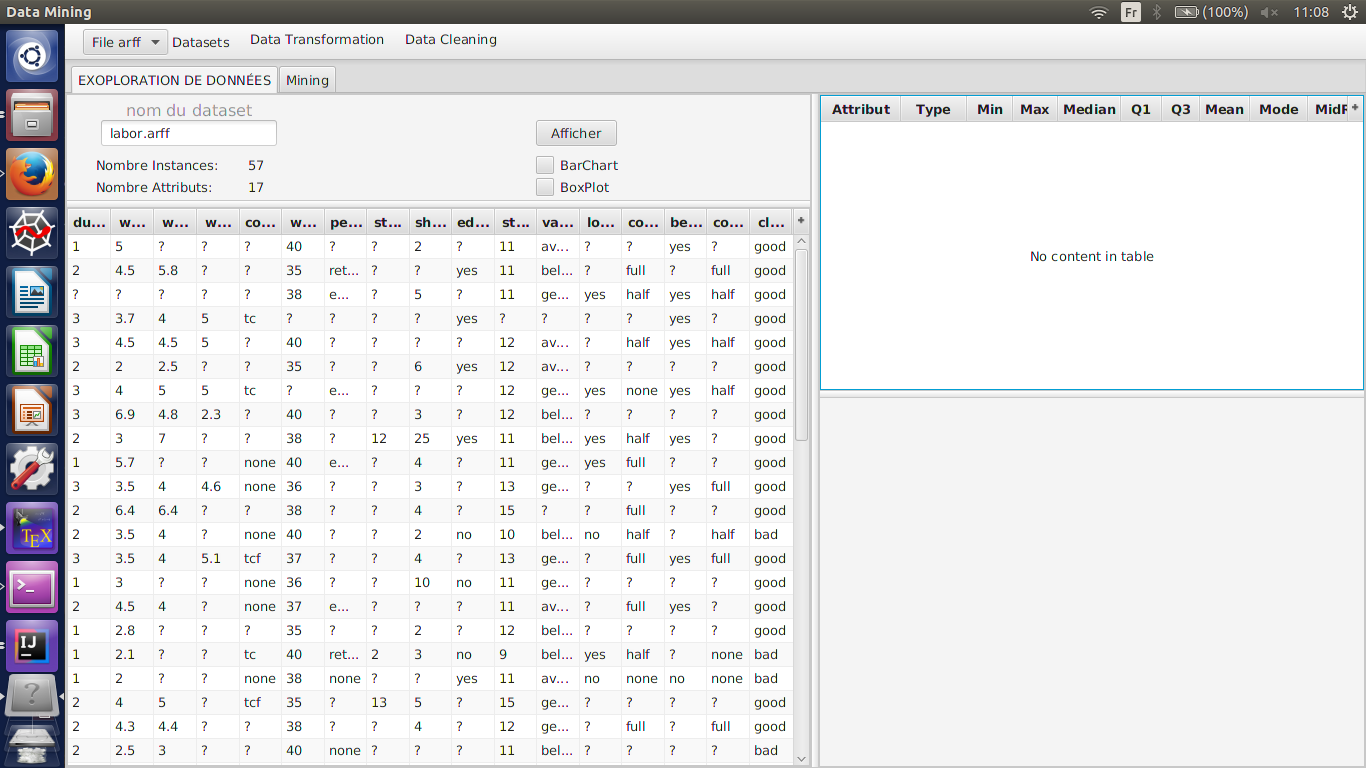
\includegraphics[width=1\textwidth]{screens/avantMissing.png}%
		\captionof{figure}{Interface de l'application affichant le Data Set [labor.arff] .}\label{labelname}%
	\end{center}
	
	
	\section{Remplacer les valeurs manquantes}
	\subsection{but}
	Remplacer les valeurs manquantes a pour principale but de redonner une certaine qualité au données, et éviter de tomber dans des cas d'inconsistance et d'incohérence par la suite dans le processus d'extraction de connaissances .
	
	\subsection{Méthode : entièrement implémenter (Orienté classe)}
	
	\textbf{Valeurs numériques :}
	
	Cette première méthode a pour principe de étant donnée une instance I ayant un attribut Ai manquant et appartenant à une classe C , on devra alors remplacer la valeur manquante de Ai par la Moyenne des valeurs des instances appartenant à la Classe C ayant une valeur dans l'attribut Ai (non manquante).
	
	\textbf{Implémentation:}
	
	Pour l'implémentation de cette méthode on a choisit de construire un dictionnaire (index) de façon à avoir: la clé c'est la Classe, les valeurs sont les instances I ayant une valeur (non manquante ) dans l'attribut Ai.
	
	\textbf{exemple: Dictionnaire pour l'attribut DURATION (numeric)}
	\begin{center}
		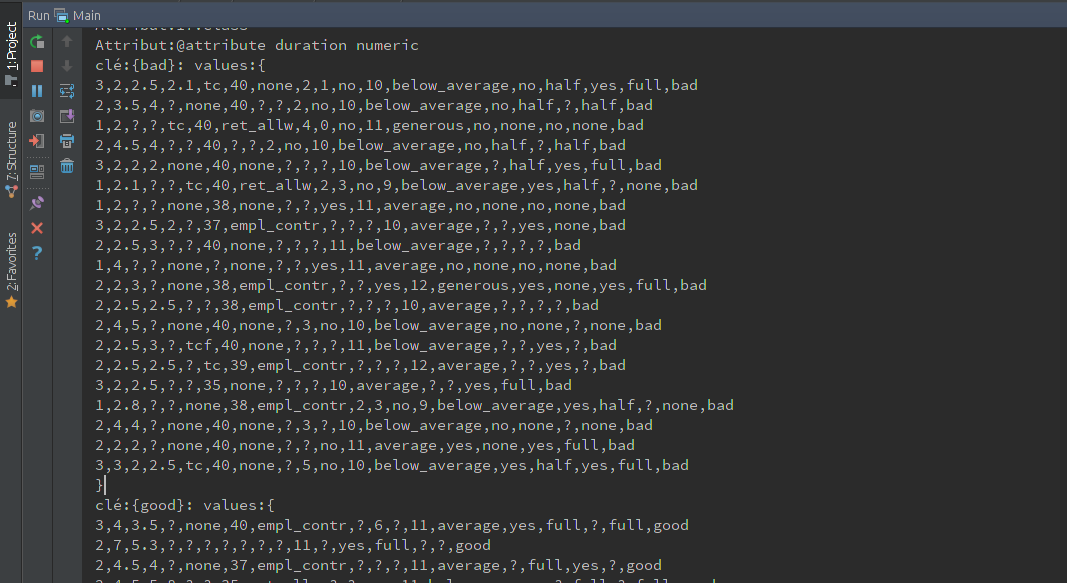
\includegraphics[width=1\textwidth]{screens/dic1.png}%
		\captionof{figure}{Dictionnaire par Classe regroupant les instances dont la valeur de l'attribut DURATION existe, Data Set [labor.arff] .}\label{labelname}%
	\end{center}
	
	\textbf{exemple: Dictionnaire pour l'attribut WAGE INCREASED EACH YEAR (numeric)}
	\begin{center}
		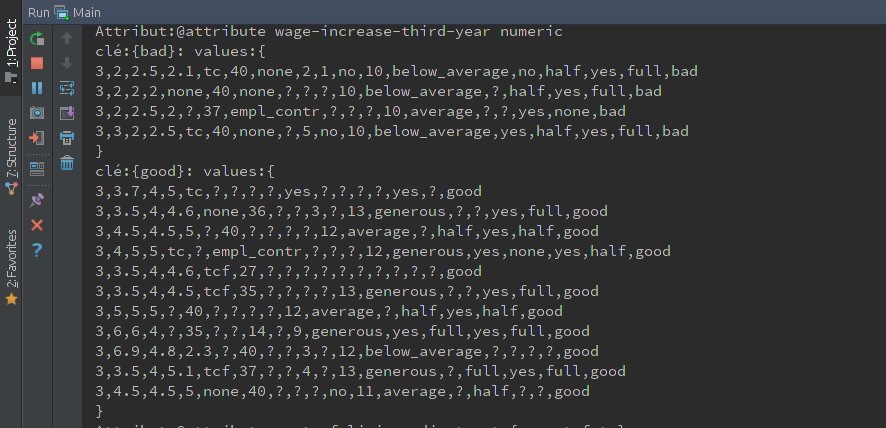
\includegraphics[width=1\textwidth]{screens/dic2.png}%
		\captionof{figure}{Dictionnaire par Classe regroupant les instances dont la valeur de l'attribut WAGE INCREASED EACH YEAR existe, Data Set [labor.arff].}\label{labelname}%
	\end{center}
	
	\textbf{Valeurs nominales:}
	Pour les valeurs nominal on choisit d'exploiter notre structure de dictionnaire et pour une instance I assigner pour chaque attribut manquant Ai appartenant à une classe C, le MODE de la Classe à laquelle l'instance Appartient (Classe C).\\
	
	\textbf{exemple: Dictionnaire pour l'attribut contribution-to-dental-plan}
	\begin{center}
		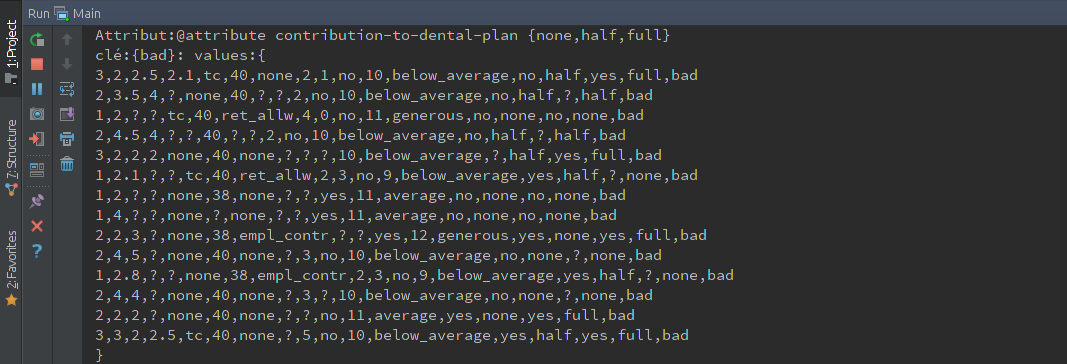
\includegraphics[width=1\textwidth]{screens/dicnominal1.png}%
		\captionof{figure}{Dictionnaire pour la classe bad regroupant les instances dont la valeur de l'attribut contribution-to-dental-plan existe, Data Set [labor.arff].}\label{labelname}%
	\end{center}
	
	
	\begin{center}
		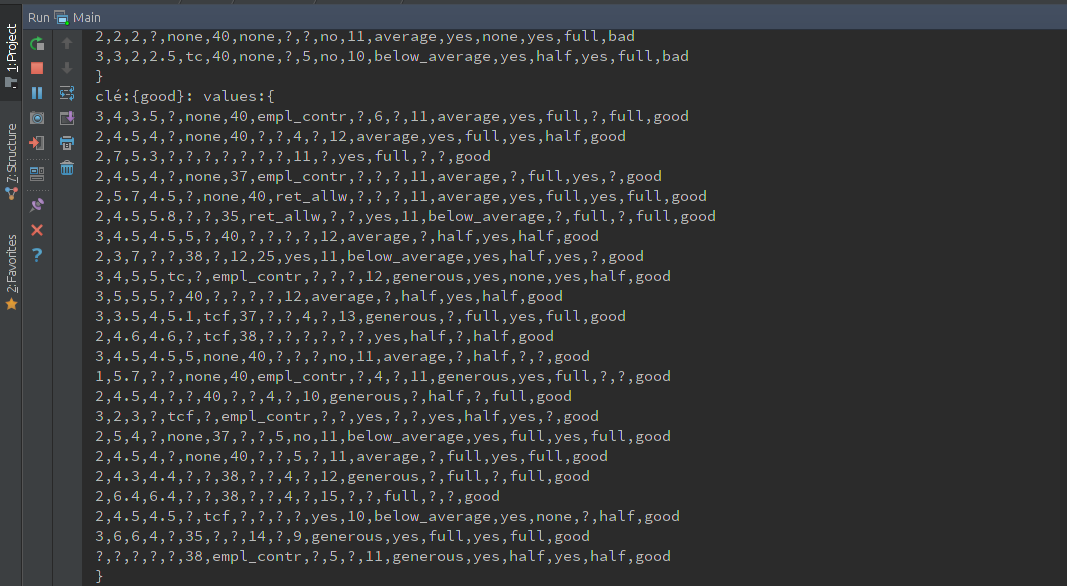
\includegraphics[width=1\textwidth]{screens/dicnominal.png}%
		\captionof{figure}{Dictionnaire pour la classe good regroupant les instances dont la valeur de l'attribut contribution-to-dental-plan existe, Data Set [labor.arff].}\label{labelname}%
	\end{center}
	
	
	\subsection{Résultat}
	Le Data Set avant de remplacer les valeurs manquantes est comme suit: 
	\begin{center}
		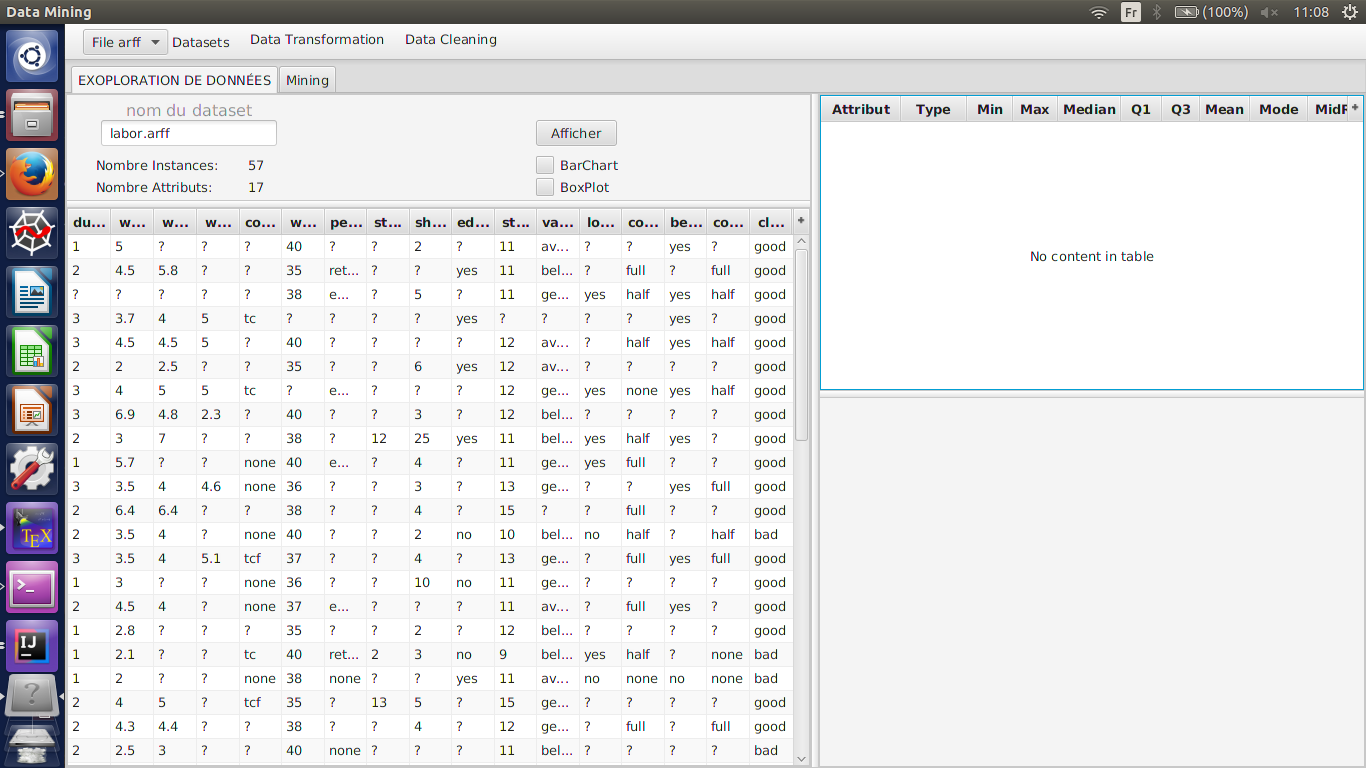
\includegraphics[width=1\textwidth]{screens/avantMissing.png}%
		\captionof{figure}{Data Set [labor.arff] avant traitement des valeurs manquantes.}\label{labelname}%
	\end{center}
	
	L'on remarque les points d'interrogation \textit{"?"} représentant les valeurs manquantes aussi bien pour les attributs nominaux que numériques.\\
	
	Après avoir sélectionné dans la barre des menus l'option \textbf{Data Cleaning $>$ Missing value class} l'on obtient le résultat suivant:
	
	\begin{center}
		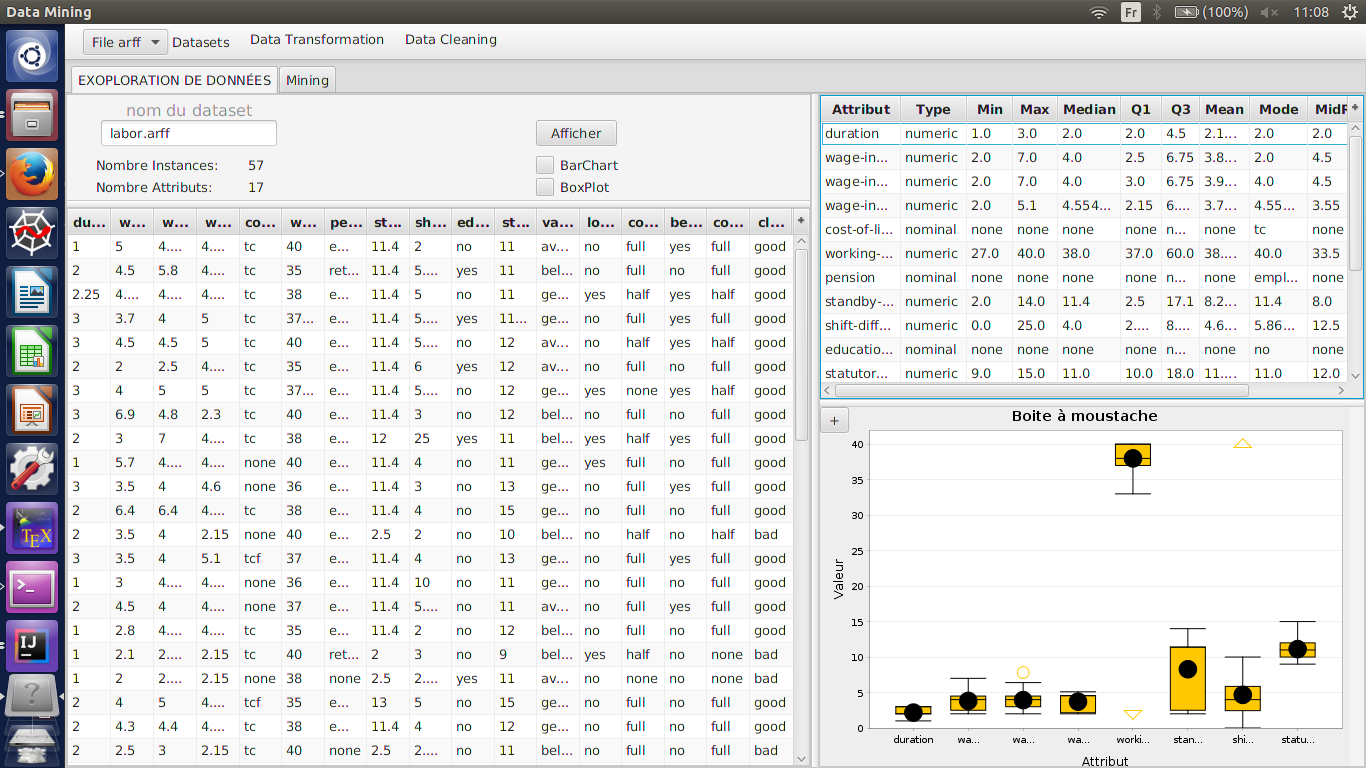
\includegraphics[width=1\textwidth]{screens/apresMissing.png}%
		\captionof{figure}{Data Set [labor.arff] après traitement des valeurs manquantes.}\label{labelname}%
	\end{center}
	
	\section{Discrétisation}
	\subsection{But[2]}
	Discrétiser un attribut numérique (à valeurs quantitatives) c'est transformer l'ensemble des valeurs réels d'un attribut en un autre ensemble réduit d'intervalles ou de classes représentatifs du premier ensemble. On dis aussi "réaliser un découpage en classes". \\
	Lorsque le nombre de valeur d'un attribut est énorme, l'affichage des histogrammes pour l'étude des caractéristiques de cet attribut est illisible, ou les informations que l'on en tire ne sont pas pertinentes, c'est pour cela que l'on à recours à la discrétisation.
	
	\subsection{Méthode}
	\subsubsection{Choix du nombre d'intervalles}
	
	Il existe quelques formules de moindre complexité pour déterminer à l'aveugle le nombre de classes à partir de:\\
	\textbf{N} : le nombre total de données.\\
	\textbf{Min} : le minimum des données.\\
	\textbf{Max} : le maximum des données.\\
	\textbf{IQR} : l'écart inter-quartiles (paramètres de la dispersion).\\
	
	Nous avons choisi la fonction de \textbf{Freedman-Diaconis} qui est la suivante:
	\begin{center}
		$NbrIntervalle = \dfrac{Max - Min}{2 * IQR * N^{-\frac{1}{3}}}$
	\end{center}
	
	
	\subsubsection{Création des intervalles/classes}
	
	Parmi plusieurs méthodes existantes nous avons opté pour \textbf{ La méthode des amplitudes} c'est à dire à tailles (amplitudes) égales.\\
	Tel que la taille de chaque intervalle est égale à:
	\begin{center}
		$Amplitude = \dfrac{(Max - Min)}{NbrIntervalle} $\\
	\end{center}
	
	\textbf{ }\\
	Ainsi en le $1^{er}$ intervalle =$[Min : Min+Amplitude]$,\\
	le suivant = [$Min+Amplitude : Min+2*Amplitude$], ... 
	
	
	\subsubsection{Remplacement de chaque valeur par la borne supérieur de l'intervalle au quel elle appartient}
	
	Ainsi pour chaque attribut , nous parcourons toutes les valeurs de celui-ci et pour chacune de ses valeur nous vérifions à quel intervalle $"I"$ elle appartient, puis nous remplaçons cette valeur par la borne supérieure de $I$.\\
	
	\underline{\textbf{PS:}} 
	L'attribut étant de type numérique et afin de ne pas dénaturer la dataset, nous avons retenu uniquement la borne supérieur des intervalles pour remplacer les valeurs lors de la discrétisation.
	
	\subsection{Résultat}
	Le Data Set avant discrétisation est comme suit: 
	\begin{center}
		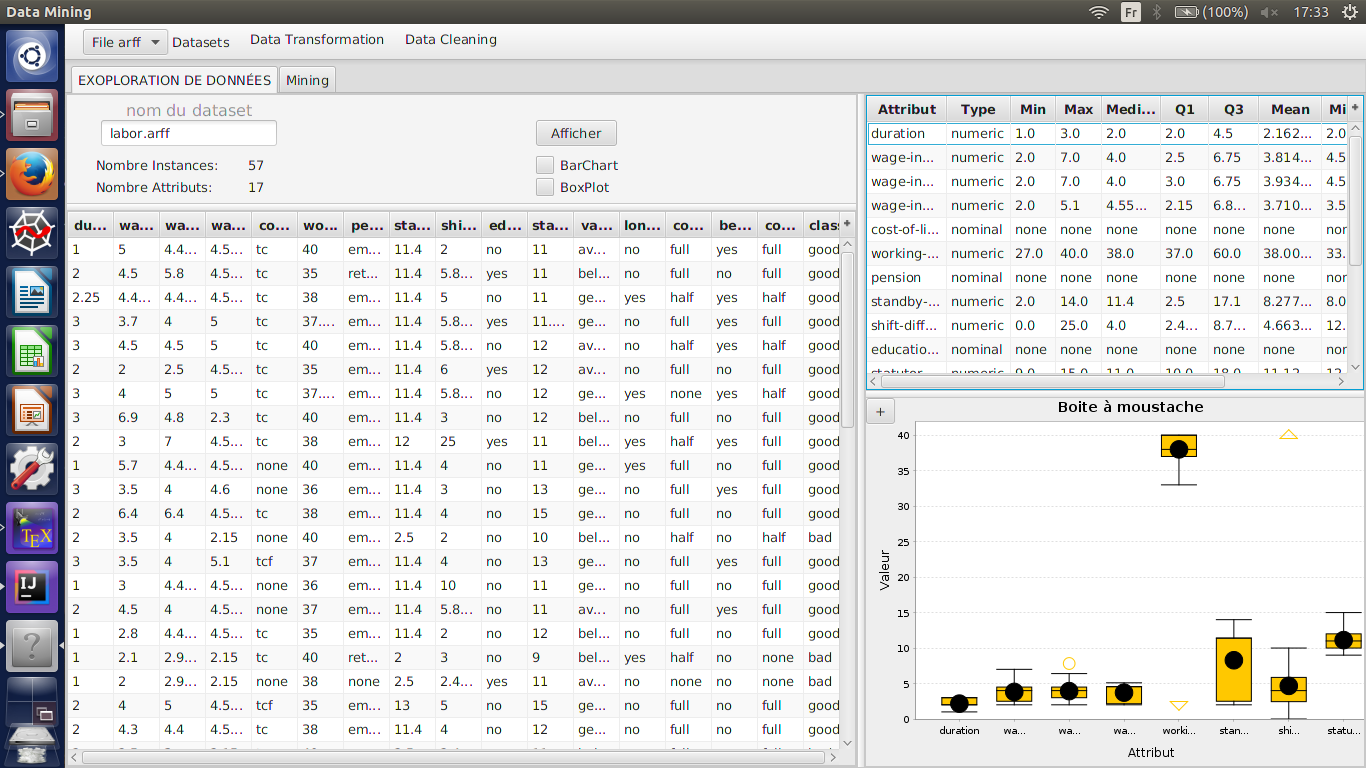
\includegraphics[width=1\textwidth]{screens/avantDiscr.png}%
		\captionof{figure}{Data Set [labor.arff] avant discrétisation.}\label{labelname}%
	\end{center}
	
	Après avoir sélectionné dans la barre des menus l'option \textbf{Data Transformation $>$ Discrétisation} l'on obtient le résultat suivant:
	
	\begin{center}
		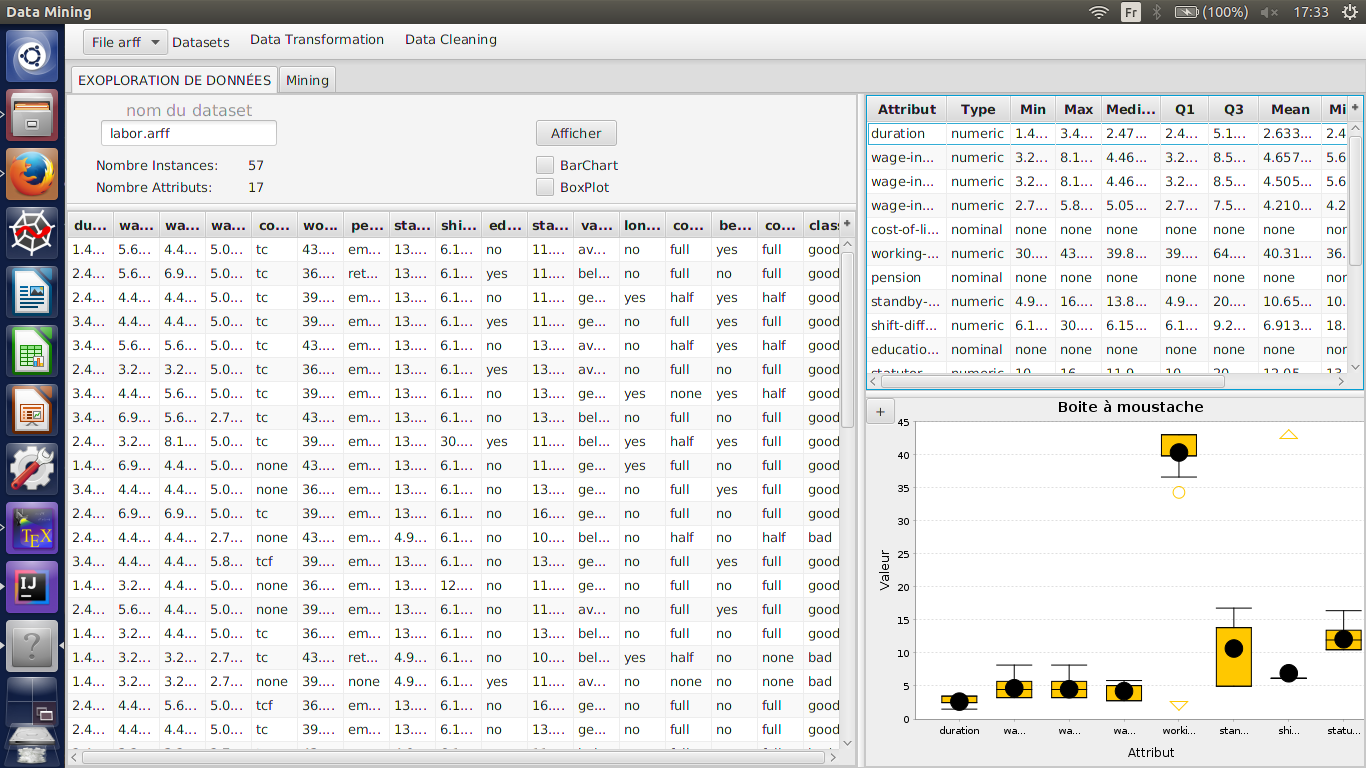
\includegraphics[width=1\textwidth]{screens/apresDiscr.png}%
		\captionof{figure}{Data Set [labor.arff] après discrétisation.}\label{labelname}%
	\end{center}
	
	\underline{\textbf{Remarque}}
	Nous remarquons ainsi que le degré de similitude entre les instances par rapport aux attributs est plus visible, ainsi nous espérons avoir de meilleurs résultats pour les prochaines étapes.
	
	
	
	\section{Normalisation}
	\subsection{But}
	
	Pour la visualisation des données, et surtout la comparaison des distributions et caractéristiques des différents attributs d'un Data Set, nous avons recours à la normalisation des données de ce dernier, car les attributs des Data Set proviennent avec des ordres de grandeurs différents.\\
	
	en plus que les attributs à grande valeur numérique influeront plus les résultats lors des traitements, apprentissage, ...
	
	\subsection{Méthode}
	Cette étape est réalisable en alignant tous les attributs sur une même plage de valeur, généralement [0:1], la formule est la suivante:
	\begin{center}
		$normalisee = \dfrac{originale - MIN}{MAX - MIN}$
	\end{center}
	\textbf{[MIN,MAX]} : intervalle d'origine.\\
	\textbf{originale} : valeur dans l'intervalle d'origine.\\
	\textbf{normalisee} : valeur normalisée dans l'intervalle cible [0,1].\\
	
	
	
	
	\subsection{résultat}
	Le Data Set avant la normalisation est comme suit: 
	\begin{center}
		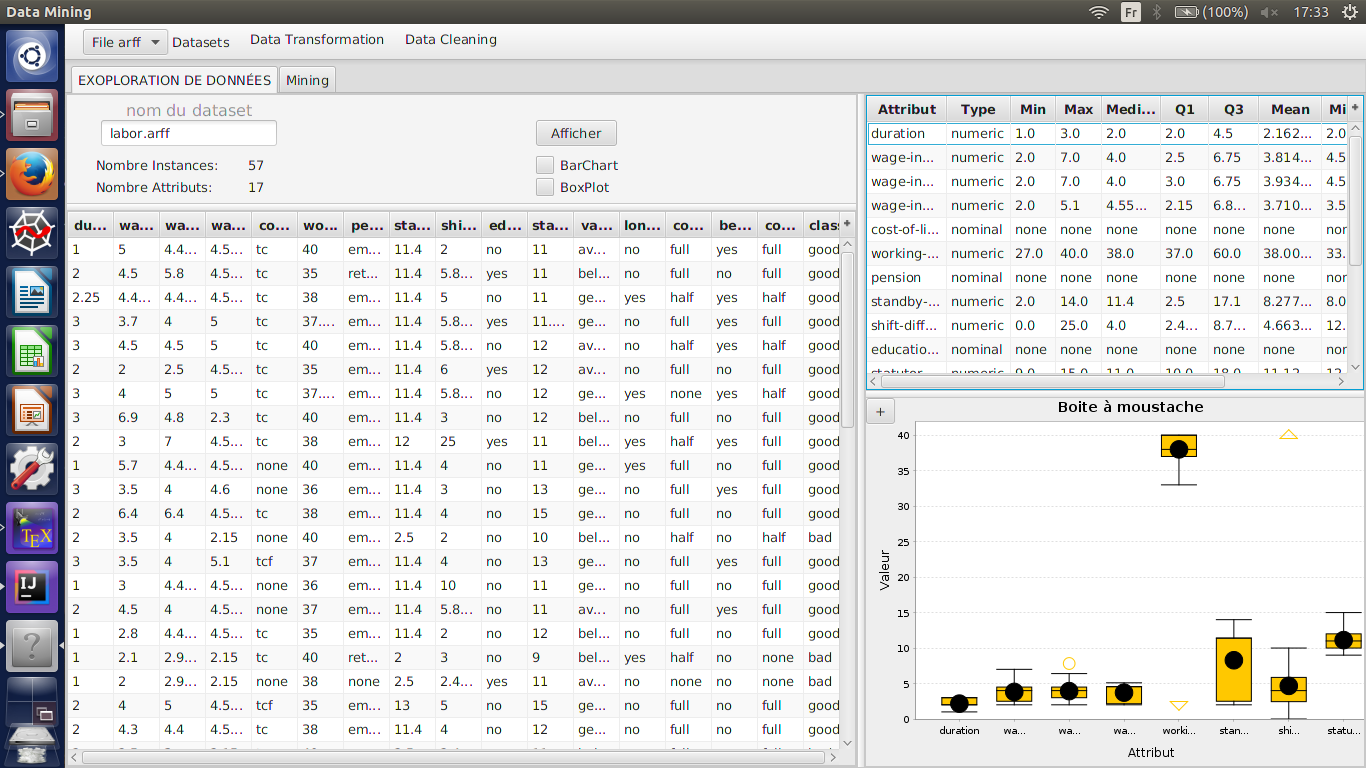
\includegraphics[width=1\textwidth]{screens/avantDiscr.png}%
		\captionof{figure}{Data Set [labor.arff] avant normalisation.}\label{labelname}%
	\end{center}
	
	Après avoir sélectionné dans la barre des menus l'option \textbf{Data Transformation $>$ Normalisation} l'on obtient le résultat suivant:
	
	\begin{center}
		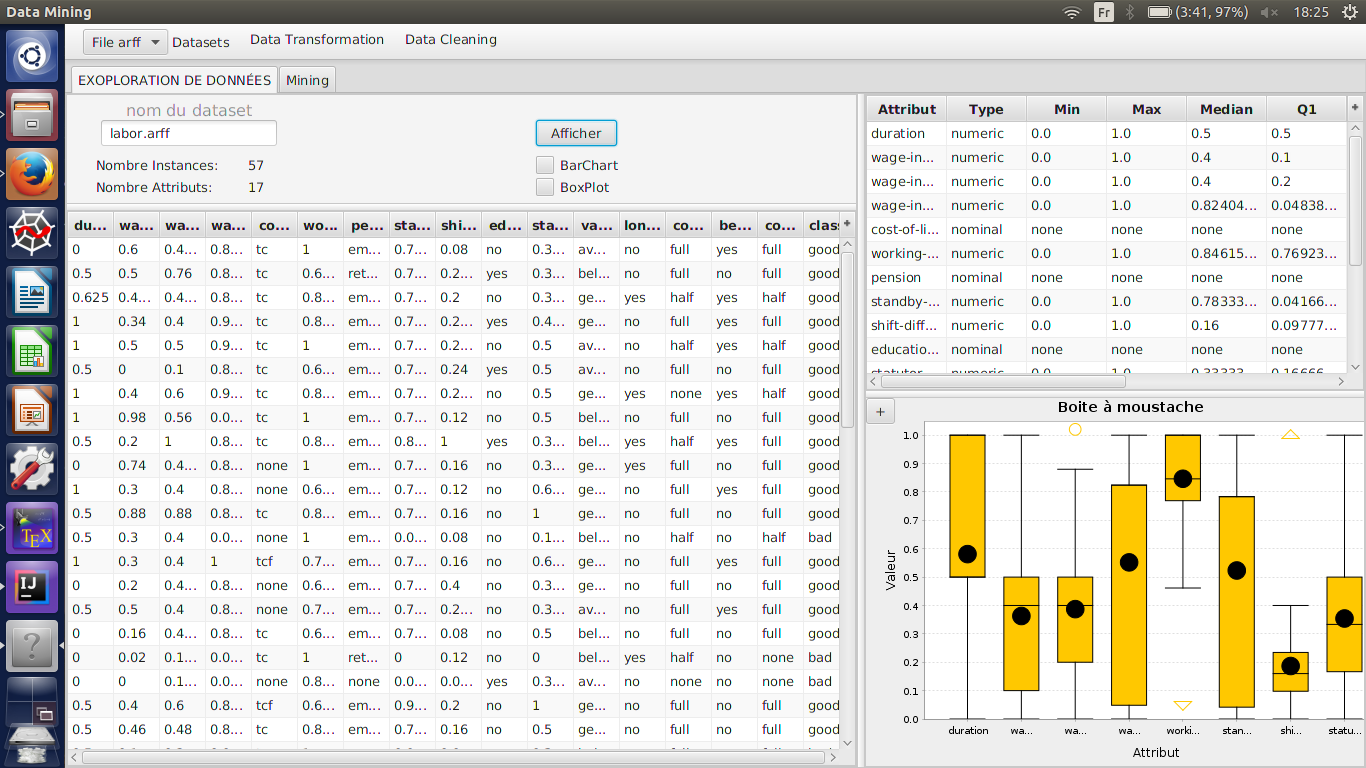
\includegraphics[width=1\textwidth]{screens/apresNormal.png}%
		\captionof{figure}{Data Set [labor.arff] après normalisation.}\label{labelname}%
	\end{center}
	
	\underline{\textbf{Remarque:}}
	Il est claire qu'il est plus simple de comparer les attributs une fois uniformisé, comme cela apparait dans l'affichage des boites à moustaches.
	
	
	
	
	
	
	\section{Description du Data Set et de ses attributs}
	Le Data Set "Labor.arff" choisi pour cette analyse comporte 16 attributs ainsi que la classe.\\
	Afin de mener à bien notre étude / analyse de ce Data Set nous aurons recours à deux moyen de visualisation qui sont les Histogramme (BarChart) ainsi que les Boites à moustache (BoxPlot), ce dernier est utilisé uniquement sur les attributs numériques, et donnée par les figures ci-dessous:
	\begin{center}
		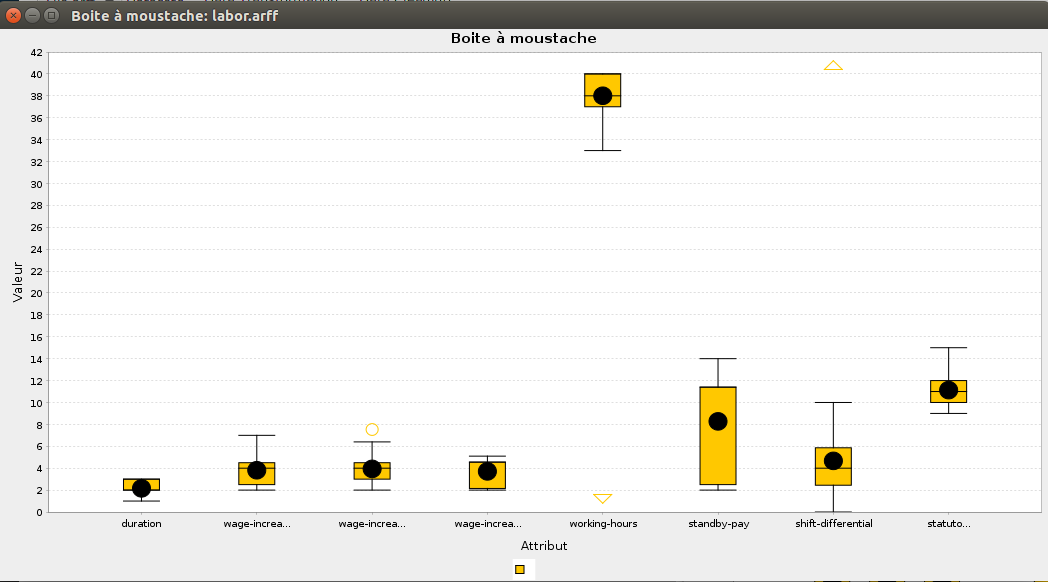
\includegraphics[width=1\textwidth]{screens/BoxPlot.png}%
		\captionof{figure}{Boites à moustaches du Data Set [labor.arff] brute.}\label{labelname}%
	\end{center}
	
	\begin{center}
		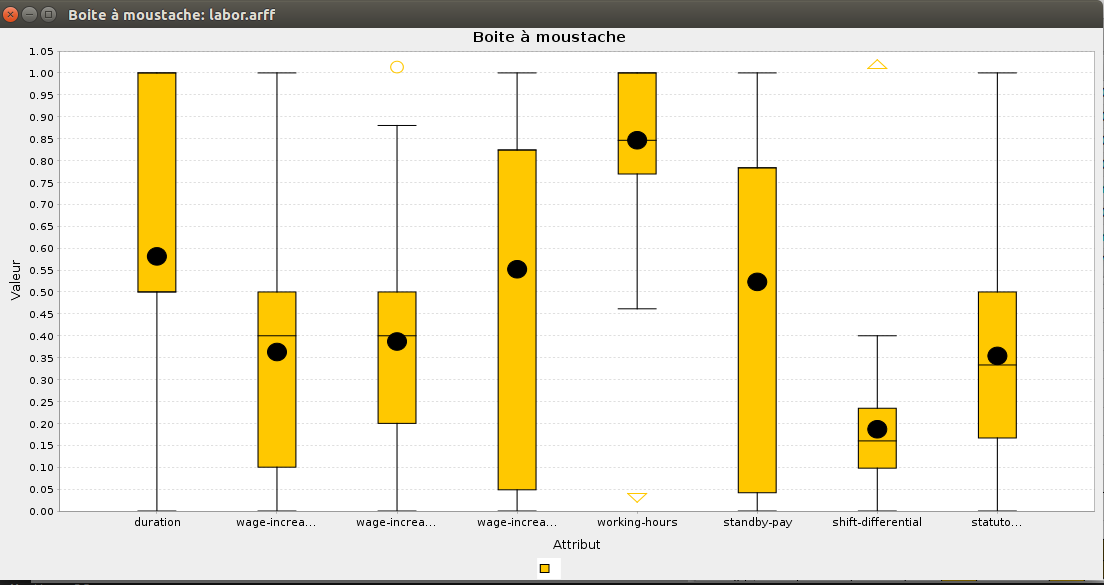
\includegraphics[width=1\textwidth]{screens/BoxPlotN.png}%
		\captionof{figure}{Boites à moustaches du Data Set [labor.arff] après normalisation.}\label{labelname}%
	\end{center}
	
	\underline{\textbf{Remarque}}
	Ces figures seront détaillées lors de la description des attributs.
	
	\newpage
	
	\subsection{Attribut 1 : duration }
	\subsubsection{Caractéristiques}
	Nous résumons les caractéristiques de cet attribut : "durée de l'accord" dans le tableau ci-dessous:
	\begin{center}
		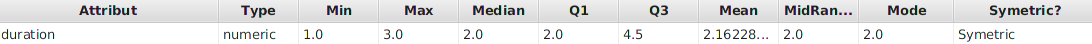
\includegraphics[width=1\textwidth]{screens/att-1.png}%
		\captionof{figure}{Attribut 1 : duration du Data Set [labor.arff] .}\label{labelname}%
	\end{center}
	On se basant sur la comparaison les valeurs de \textit{[Mode , Médiane , Moyenne] = (2 , 2 , 2.1)}, nous déduisons la dispersion des données selon cet attribut, tel qu'il est \textbf{Symétrique}.
	
	\subsubsection{BarChart}
	
	\begin{center}
		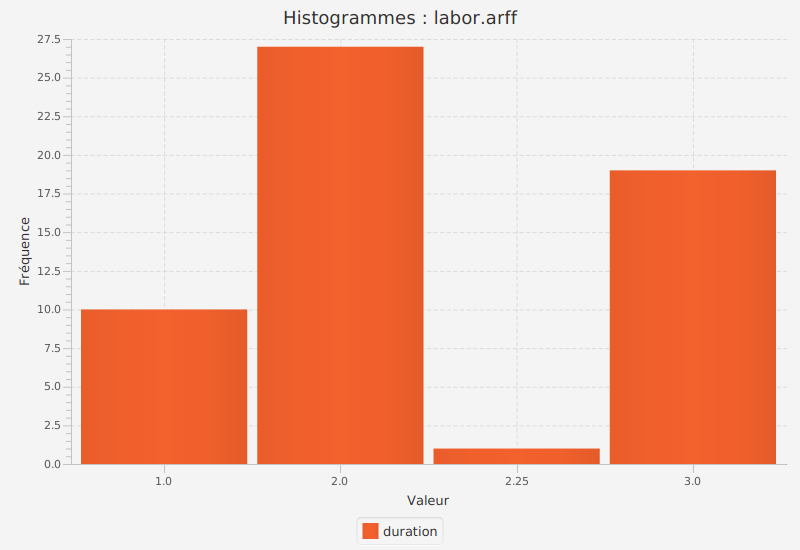
\includegraphics[width=0.8\textwidth]{screens/barchart/duration-barchart.png}%
		\captionof{figure}{Histogramme de duration du Data Set [labor.arff] .}\label{labelname}%
	\end{center}
	
	\subsubsection{discussion}
	$\bullet $ L'on remarque que cet attribut peut prendre 4 valeurs possibles \textit{(1.0 , 2.0 , 2.25 , 3.0)}. la répartition n'est pas uniforme vu la fréquence d'apparition de la valeur \textit{(2.25)} comparé à celle de la valeur \textit{(2.0)}.\\
	\textbf{ }\\
	$\bullet $ Il est aussi à noter que cet attribut est \textbf{Uni-modal}, tel que mode = \textit{(2.0)}.\\
	\textbf{ }\\
	$\bullet $ A travers sa boite à moustache de cet attribut nous constatons une répartition pas très uniforme des données, dans le sens ou il y a une concentration des données pour les valeurs supérieurs entre (2.0 , 3.0).
	
	
	\newpage
	
	
	\subsection{Attribut 2 : wage-increase-first-year }
	\subsubsection{Caractéristiques}
	Nous résumons les caractéristiques de cet attribut : "augmentation en première année de contrat" dans le tableau ci-dessous:
	\begin{center}
		
\includegraphics[width=1\textwidth]{screens/att.png}\\
		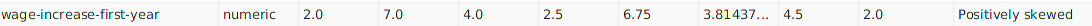
\includegraphics[width=1\textwidth]{screens/att-2.png}%
		\captionof{figure}{Attribut 2 : wage-increase-first-year du Data Set [labor.arff] .}\label{labelname}%
	\end{center}
	
	On se basant sur la comparaison les valeurs de \textit{[Mode , Médiane , Moyenne] = (2.0 , 4.0 , 3.81)}, nous déduisons la dispersion des données selon cet attribut, tel qu'il est \textbf{asymétrique positivement}.
	
	\subsubsection{BarChart}
	
	\begin{center}
		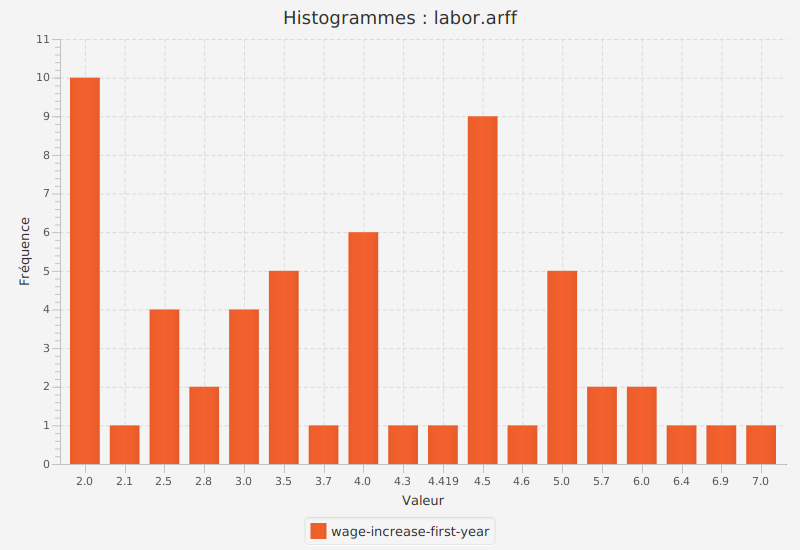
\includegraphics[width=0.8\textwidth]{screens/barchart/wage-increase-first-year-barchart.png}%
		\captionof{figure}{Histogramme de wage-increase-first-year du Data Set [labor.arff] .}\label{labelname}%
	\end{center}
	
	\subsubsection{discussion}							
	$\bullet $ L'on remarque que cet attribut peut prendre 18 valeurs possibles \textit{(2.0 , 2.1 , 2.5 , 2.8 , 3.0 , 3.5 , 3.7 , 4.0 , 4.3 , 4.419 , 4.5 , 4.6 , 5.0 , 5.7 , 6.0 , 6.4 , 6.9 , 7.0)}. la répartition n'est pas uniforme vu par exemple : la fréquence d'apparition de la valeur \textit{(7.0)} comparé à celle de la valeur \textit{(2.0)} ou de la valeur \textit{(4.5)}.\\
	\textbf{ }\\
	$\bullet $ Il est aussi à noter que cet attribut est \textbf{Uni-modal}, tel que mode = \textit{(2.0)}.\\
	\textbf{ }\\
	$\bullet $ A travers sa boite à moustache de cet attribut nous constatons une répartition plus ou moins uniforme des données, mis à part une légère tendance vers les valeurs inférieur.
	
	
	\newpage
	
	
	\subsection{Attribut 3 : wage-increase-second-year }
	\subsubsection{Caractéristiques}
	Nous résumons les caractéristiques de cet attribut : "augmentation en deuxième année de contrat" dans le tableau ci-dessous:
	\begin{center}
		
\includegraphics[width=1\textwidth]{screens/att.png}\\ 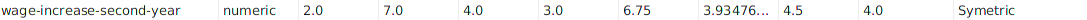
\includegraphics[width=1\textwidth]{screens/att-3.png}%
		\captionof{figure}{Attribut 3 : wage-increase-second-year du Data Set [labor.arff] .}\label{labelname}%
	\end{center}
	
	On se basant sur la comparaison les valeurs de \textit{[Mode , Médiane , Moyenne] = (4.0 , 4.0 , 3.93)}, nous déduisons la dispersion des données selon cet attribut, tel qu'il est \textbf{symétrique}.
	
	\subsubsection{BarChart}
	
	\begin{center}
		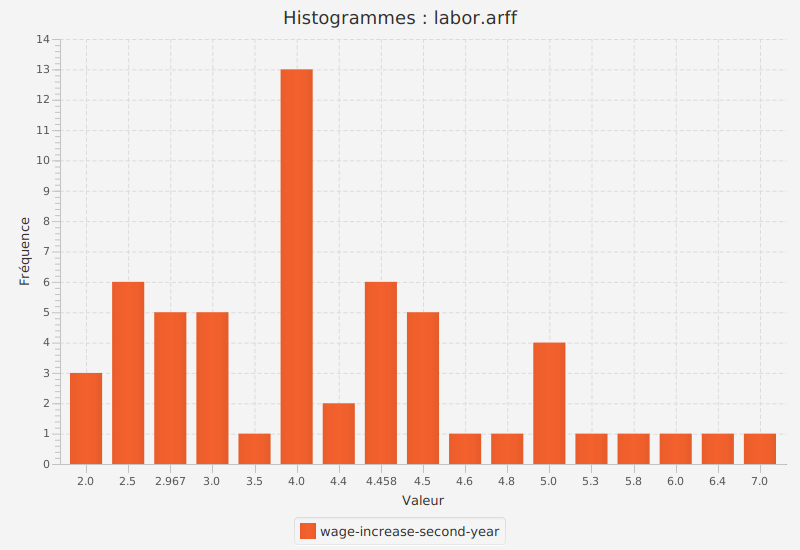
\includegraphics[width=0.8\textwidth]{screens/barchart/wage-increase-second-year-barchart.png}%
		\captionof{figure}{Histogramme de wage-increase-second-year du Data Set [labor.arff] .}\label{labelname}%
	\end{center}	
	
	\subsubsection{discussion}	
	$\bullet $ L'on remarque que cet attribut peut prendre 16 valeurs possibles \textit{(2.0 , 2.5 , 2.967 , 3.0 , 3.5 , 4.0 , 4.4 , 4.458 , 4.6 , 4.8 , 5.0 , 5.3 , 5.8  , 6.0 , 6.4 , 7.0)}. la répartition n'est pas uniforme vu par exemple : la fréquence d'apparition de la valeur \textit{(7.0)} comparé à celle de la valeur \textit{(4.0)}.\\
	\textbf{ }\\
	$\bullet $ Il est aussi à noter que cet attribut est \textbf{Uni-modal}, tel que mode = \textit{(4.0)}.\\
	\textbf{ }\\
	$\bullet $ La boite à moustache de cet attribut nous permet de remarquer que la distribution des valeurs n'est pas tout à fait uniforme, tel que plusieurs valeur assez grandes n'apparaissent qu'une fois dans tous le Data Set, ce qui signifie qu'elles peuvent être considérées comme des valeurs aberrantes (out-liers).
	
	\newpage
	
	
	\subsection{Attribut 4 : wage-increase-third-year }
	\subsubsection{Caractéristiques}
	Nous résumons les caractéristiques de cet attribut : "augmentation en troisième année de contrat" dans le tableau ci-dessous:
	\begin{center}
		
\includegraphics[width=1\textwidth]{screens/att.png}\\ 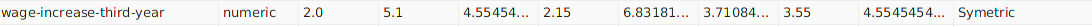
\includegraphics[width=1\textwidth]{screens/att-4.png}%
		\captionof{figure}{Attribut 4 : wage-increase-third-year du Data Set [labor.arff] .}\label{labelname}%
	\end{center}
	
	On se basant sur la comparaison les valeurs de \textit{[Mode , Médiane , Moyenne] = (4.0 , 4.0 , 3.93)}, nous déduisons la dispersion des données selon cet attribut, tel qu'il est \textbf{symétrique}.
	
	\subsubsection{BarChart}
	
	\begin{center}
		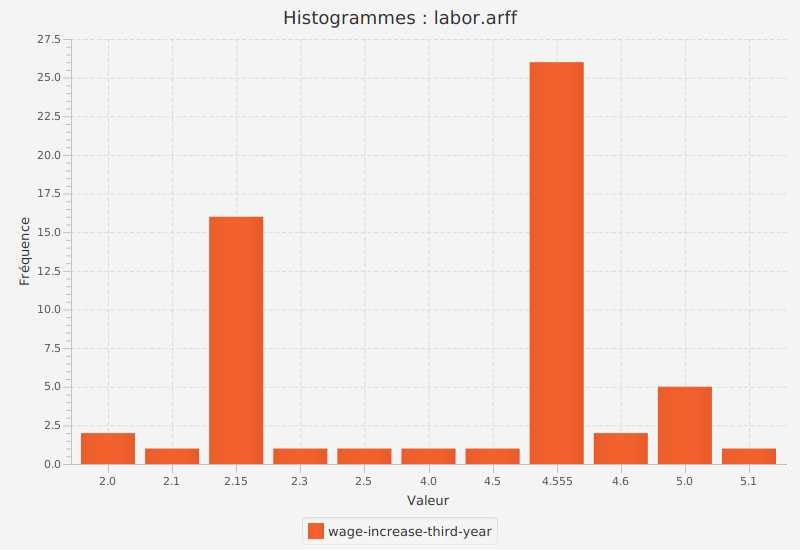
\includegraphics[width=0.8\textwidth]{screens/barchart/wage-increase-third-year-barchart.png}%
		\captionof{figure}{Histogramme de wage-increase-third-year du Data Set [labor.arff] .}\label{labelname}%
	\end{center}
	
	\subsubsection{discussion}
	$\bullet $ L'on remarque que cet attribut peut prendre 11 valeurs possibles \textit{(2.0 , 2.1 , 2.15 , 2.3 , 2.5 , 4 , 4.5 , 4.555 , 4.6 , 5.0 , 5.1)}. la répartition n'est pas uniforme vu par exemple : la fréquence d'apparition de la valeur \textit{(5.1)} comparé à celle de la valeur \textit{(2.15)}.\\
	\textbf{ }\\
	$\bullet $ Il est aussi à noter que cet attribut est \textbf{Uni-modal}, tel que mode = \textit{(4.555)}.\\
	\textbf{ }\\
	$\bullet $ La boite à moustache de cet attribut nous permet d'apprécier la distribution uniforme de ses valeurs, ainsi aucune valeur aberrante n'y
	figure.
	
	
	\newpage
	
	\subsection{Attribut 5 : cost-of-living-adjustment }
	\subsubsection{Caractéristiques}
	Nous résumons les caractéristiques de cet attribut dans le tableau ci-dessous:
	\begin{center}
		
\includegraphics[width=1\textwidth]{screens/att.png}\\ 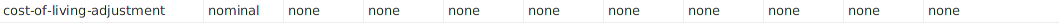
\includegraphics[width=1\textwidth]{screens/att-5.png}%
		\captionof{figure}{Attribut 5 : cost-of-living-adjustment du Data Set [labor.arff] .}\label{labelname}%
	\end{center}
	
	\subsubsection{BarChart}
	\begin{center}
		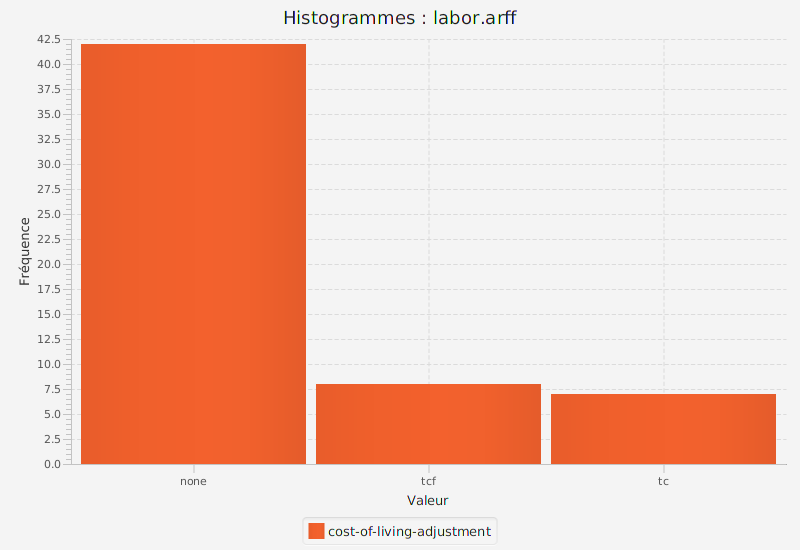
\includegraphics[width=0.8\textwidth]{screens/barchart/cost-of-living-adjustment-barchart.png}%
		\captionof{figure}{Histogramme de cost-of-living-adjustment du Data Set [labor.arff] .}\label{labelname}%
	\end{center}
	\subsubsection{discussion}
	$\bullet$ On remarque ici facilement que la valeur la plus fréquente est la \textbf{"none"} ,avec environ 70\% du tout le data set , on retrouve \textbf{"tcf","tc"} avec seulement 12\% chacun.\\
	\textbf{ }\\
	$\bullet$ On peut conclure que l'attribut est \textbf{Uni-modal }(NOne est le mode et il est unique), de plus la distribution n'est pas uniforme  tel que deux valeurs \textbf{(none)} prend le dessus sur plus de 70\% de tout le Data Set.
	
	
	\newpage
	
	\subsection{Attribut 6 : working-hours }
	\subsubsection{Caractéristiques}
	Nous résumons les caractéristiques de cet attribut : "nombre d'heure de travail" dans le tableau ci-dessous:
	\begin{center}
		
\includegraphics[width=1\textwidth]{screens/att.png}\\ 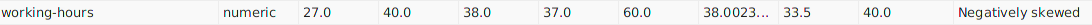
\includegraphics[width=1\textwidth]{screens/att-6.png}%
		\captionof{figure}{Attribut 6 : working-hours du Data Set [labor.arff] .}\label{labelname}%
	\end{center}
	On se basant sur la comparaison les valeurs de \textit{[Mode , Médiane , Moyenne] = (40.0 , 38.0 , 38.002)}, nous déduisons la dispersion des données selon cet attribut, tel qu'il est légèrement \textbf{asymétrique négativement}.
	
	\subsubsection{BarChart}
	\begin{center}
		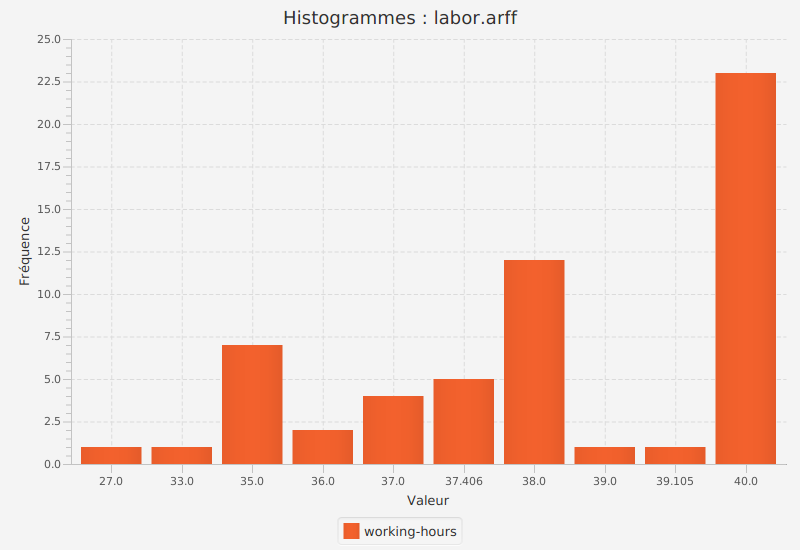
\includegraphics[width=0.8\textwidth]{screens/barchart/working-hours-barchart.png}%
		\captionof{figure}{Histogramme de working-hours du Data Set [labor.arff] .}\label{labelname}%
	\end{center}
	\subsubsection{discussion}
	$\bullet $ L'on remarque que cet attribut peut prendre 10 valeurs possibles \textit{(27.0 , 33.0 , 35.0 , 36.0 , 37.0 , 37.406 , 38.0 , 39.0 , 39.105 , 40.0)}. la répartition n'est pas uniforme vu par exemple la fréquence d'apparition de la valeur \textit{(40.0)} comparé à celle de la valeur \textit{(27.0)}.\\
	\textbf{ }\\
	$\bullet $ Il est aussi à noter que cet attribut est \textbf{Uni-modal}, tel que l'unique mode = \textit{(40.0)}.\\
	\textbf{ }\\
	$\bullet $ Aussi à partir de la boite à moustache de cet attribut, nous observons que l'ensemble des données (instances) est concentré entre (37.0 , 40.0) hors que le min est de 27h qui n'apparait qu'une seule fois, d'ailleurs se détail est bien représenté dans la boite à moustache par une flèche orange vers le bas, cela signifie la présence de valeur aberrante (out-lier). 
	
	\newpage
	
	
	\subsection{Attribut 7 : pension }
	\subsubsection{Caractéristiques}
	Nous résumons les caractéristiques de cet attribut : "contribution des employées à la pension" dans le tableau ci-dessous:
	\begin{center}
		
\includegraphics[width=1\textwidth]{screens/att.png}\\ 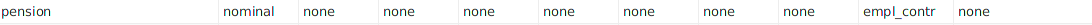
\includegraphics[width=1\textwidth]{screens/att-7.png}%
		\captionof{figure}{Attribut 7 : pension du Data Set [labor.arff] .}\label{labelname}%
	\end{center}
	
	\subsubsection{BarChart}
	\begin{center}
		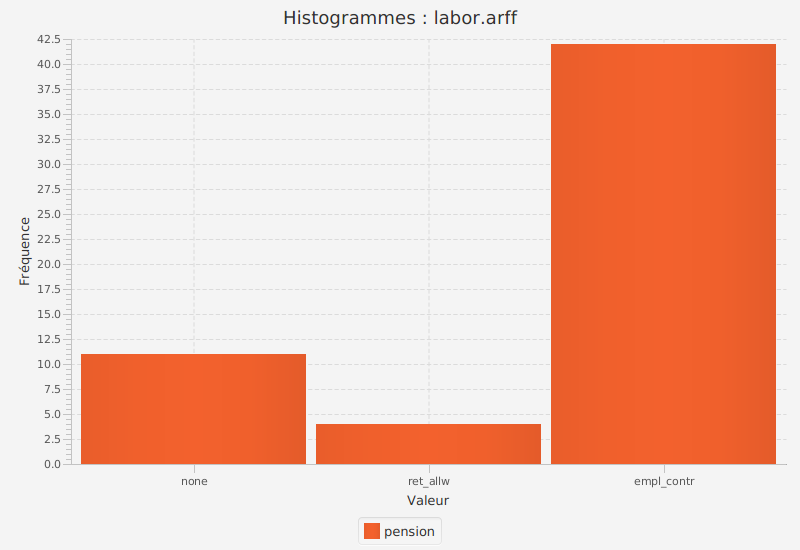
\includegraphics[width=0.8\textwidth]{screens/barchart/pension-barchart.png}%
		\captionof{figure}{Histogramme de pension du Data Set [labor.arff] .}\label{labelname}%
	\end{center}
	\subsubsection{discussion}
	$\bullet$ Comme vu plus haut l'attribut pension(contribution des employées à la pension) a trois valeurs possible (none,ret\_allw(retraité),empl\_contr), \textbf{empl\_contr} étant la plus fréquente avec  75\% , suivie de \textbf{none} (aucune valeur)
	à 17\% et plus rarement (ret\_allw) ayant 4\% seulement.\\
	\textbf{ }\\
	$\bullet$ Pension est alors uni-modal(avec empl\_contr) qui contribue le plus  au plan pension, et les retraités beaucoup moins avec seulement 4\%, ceux qui restent ne contribuent pas du tout au plan pension (none).
	
	\newpage
	
	\subsection{Attribut 8 : standby-pay }
	\subsubsection{Caractéristiques}
	Nous résumons les caractéristiques de cet attribut : "rémunération au repos" dans le tableau ci-dessous:
	\begin{center}
		
\includegraphics[width=1\textwidth]{screens/att.png}\\ 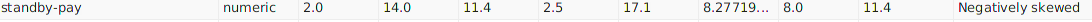
\includegraphics[width=1\textwidth]{screens/att-8.png}%
		\captionof{figure}{Attribut 8 : standby-pay du Data Set [labor.arff] .}\label{labelname}%
	\end{center}
	
	
	\subsubsection{BarChart}
	\begin{center}
		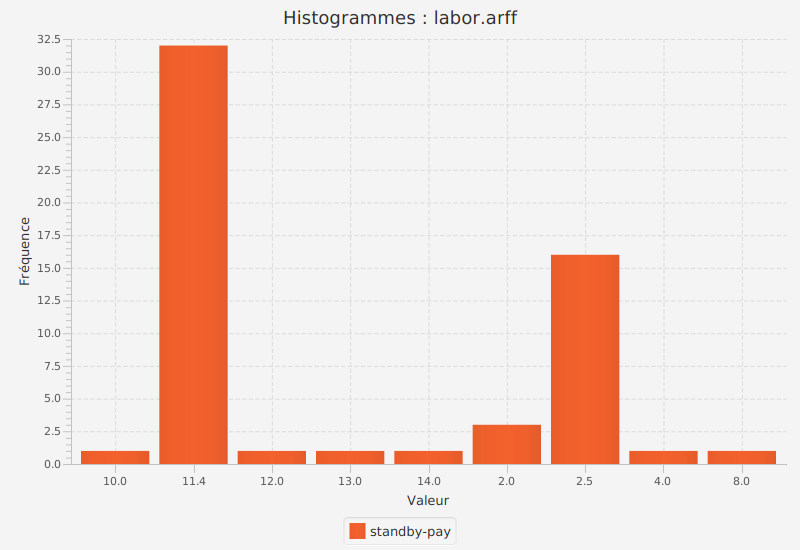
\includegraphics[width=0.8\textwidth]{screens/barchart/standby-pay-barchart.png}%
		\captionof{figure}{Histogramme de standby-pay du Data Set [labor.arff] .}\label{labelname}%
	\end{center}
	
	\subsubsection{discussion}
	$\bullet$ L'attribut standby-pay est numérique ,d'aprés l'histogramme de distribution des valeurs on remarque qu'il est uni-modal et la valeur la plus fréquente est de 11.4 suivie de 2.5, à noter que c'est les valeurs calculées auparavant lors des bourrages des valeurs manquantes , on peut déduire alors que avant nettoyage de données l'attribut avait pour mode 2.0 .\\
	\textbf{ }\\
	$\bullet$ Les valeurs de l'attribut varie entre min 2.0 jusqu'à max 14 ,en observant la boite à moustache on peut voir que la distribution des données est du coté gauche de la médiane ce qui se confirme avec moyenne < à la médiane == mode , le max 14 est ici considéré comme out-lier .
	ceci nous permet de conclure que Standby-pay est un attribut positivement symétrique .
	
	\newpage
	
	
	\subsection{Attribut 9 : shift-differential }
	\subsubsection{Caractéristiques}
	Nous résumons les caractéristiques de cet attribut : "supplément pour travail sur les équipes II et III" dans le tableau ci-dessous:
	\begin{center}
		
\includegraphics[width=1\textwidth]{screens/att.png}\\ 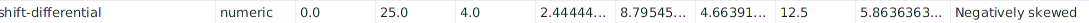
\includegraphics[width=1\textwidth]{screens/att-10.png}%
		\captionof{figure}{Attribut 9 : shift-differential du Data Set [labor.arff] .}\label{labelname}%
	\end{center}
	
	\subsubsection{BarChart}
	\begin{center}
		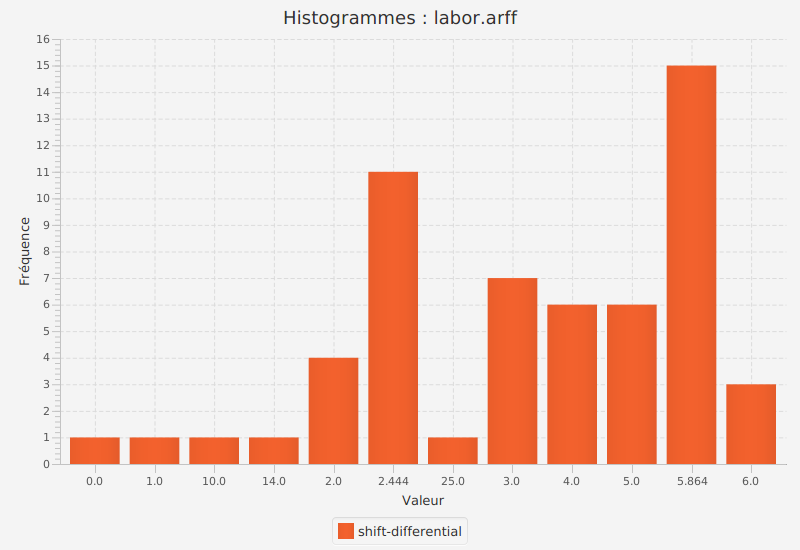
\includegraphics[width=0.8\textwidth]{screens/barchart/shift-differential-barchart.png}%
		\captionof{figure}{Histogramme de shift-differential du Data Set [labor.arff] .}\label{labelname}%
	\end{center}
	
	\subsubsection{discussion}
	$\bullet$ L'attribut shift-differential (supplément de travail sur poste 1 , 2 (travail pendant les vacances)...) est numérique ,d'après l'histogramme de distribution des valeurs on remarque facilement qu'il est uni-modal , avec 3 comme unique mode avant nettoyage des données puis 5.8 après bourrages des valeurs manquantes, par contre d'âpres la boite à moustache on observe que la distribution des données (instances) est plutôt loin des min et max qui sont de 0 et 25 respectivement. \\
	
	25  peut être considéré comme valeur aberrante(out-lier) il n'apparaît qu'une seule fois (une seule instance) et il est très loin de la moyenne et la médiane ainsi que du mode (5.8).\\
	\textbf{ }\\
	$\bullet$ la médiane étant inférieur à la moyenne et la moyenne au mode  donc l'attribut a une distribution qui  est légèrement symétrique négativement tel que la plus part des données se concentre après la médiane coté gauche.
	
	
	\newpage
	
	
	\subsection{Attribut 10 : education-allowance}
	\subsubsection{Caractéristiques}
	Nous résumons les caractéristiques de cet attribut : "allocation d'éducation" dans le tableau ci-dessous:
	\begin{center}
		
\includegraphics[width=1\textwidth]{screens/att.png}\\ 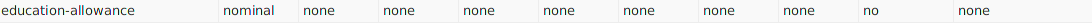
\includegraphics[width=1\textwidth]{screens/att-9.png}%
		\captionof{figure}{Attribut 10 : education-allowance du Data Set [labor.arff] .}\label{labelname}%
	\end{center}
	
	\subsubsection{BarChart}
	\begin{center}
		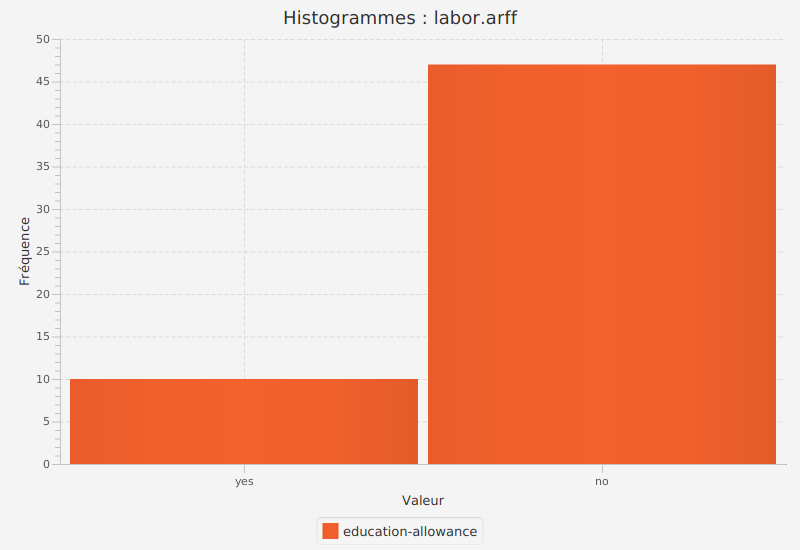
\includegraphics[width=0.8\textwidth]{screens/barchart/education-allowance-barchart.png}%
		\captionof{figure}{Histogramme de education-allowance du Data Set [labor.arff] .}\label{labelname}%
	\end{center}
	
	\subsubsection{discussion}
	$\bullet$ L'attribut education-allowance est binaire soit oui, ou non (bourses données par l'employeur à l'employé) .On remarque que dans 84\%  des on ne donne pas d'education-allowance  par contre  seulement \%16  ont droit à une education-allowance.\\
	\textbf{ }\\
	$\bullet$ On conclue que "education-allowance" est uni-modal avec la valeur ("NO") la plus fréquente.
	
	
	\newpage
	
	\subsection{Attribut 11 : statutory-holidays}
	\subsubsection{Caractéristiques}
	Nous résumons les caractéristiques de cet attribut : "nombre de jours fériés" dans le tableau ci-dessous:
	\begin{center}
		
\includegraphics[width=1\textwidth]{screens/att.png}\\ 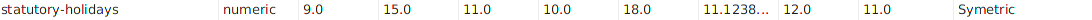
\includegraphics[width=1\textwidth]{screens/att-11.png}%
		\captionof{figure}{Attribut 11 : statutory-holidays du Data Set [labor.arff] .}\label{labelname}%
	\end{center}
	
	\subsubsection{BarChart}
	\begin{center}
		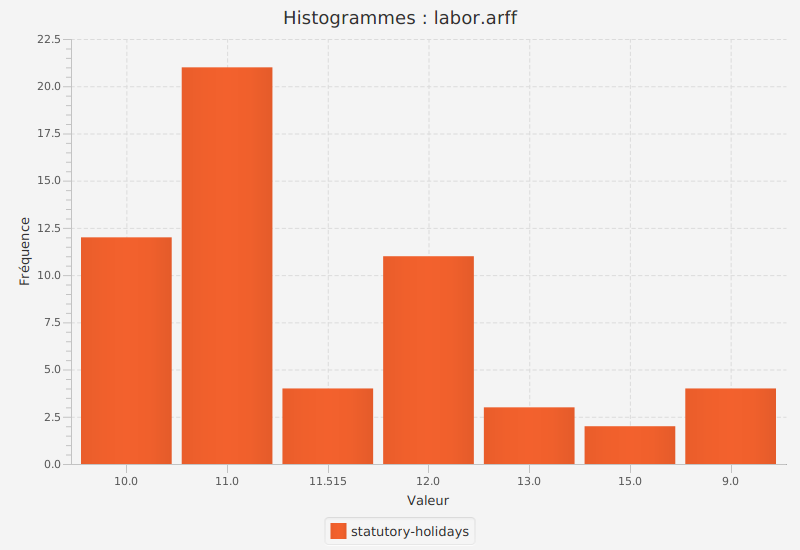
\includegraphics[width=0.8\textwidth]{screens/barchart/statutory-holidays-barchart.png}%
		\captionof{figure}{Histogramme de statutory-holidays du Data Set [labor.arff] .}\label{labelname}%
	\end{center}
	
	\subsubsection*{discussion}
	
	
	$\bullet$ L'attribut statutory holidays est representatif des nombres en jours de vacances permises, on remarque que il varie entre min=10 et max=15 , d'après la répartition des données sur l'histogramme on peut interpréter l'existence d'un seul mode qui est : 11 ce qui implique attribut $\Rightarrow$ (uni-modal) ainsi que 10 et 11 ,13 couvre plus de la moitié (prés de 77\%) de toutes la distribution des données.\\
	\textbf{ }\\
	$\bullet$ Maintenant à partir de la boite à moustache on peut facilement noter que la médiane et la moyenne sont égales , leur valeur étant 11 qui est aussi la valeur du mode cella nous permet de conclure que la distribution des données selon l'attribut "statutory holidays " est symétrique . (uniforme) 
	
	\newpage
	
	\subsection{Attribut 12 : vacation}
	\subsubsection{Caractéristiques}
	Nous résumons les caractéristiques de cet attribut : "nombre de jours de congés payés" dans le tableau ci-dessous:
	\begin{center}
		
\includegraphics[width=1\textwidth]{screens/att.png}\\ 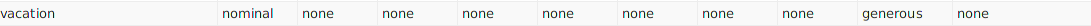
\includegraphics[width=1\textwidth]{screens/att-13.png}%
		\captionof{figure}{Attribut 12 : vacation du Data Set [labor.arff] .}\label{labelname}%
	\end{center}
	
	\subsubsection{BarChart}
	\begin{center}
		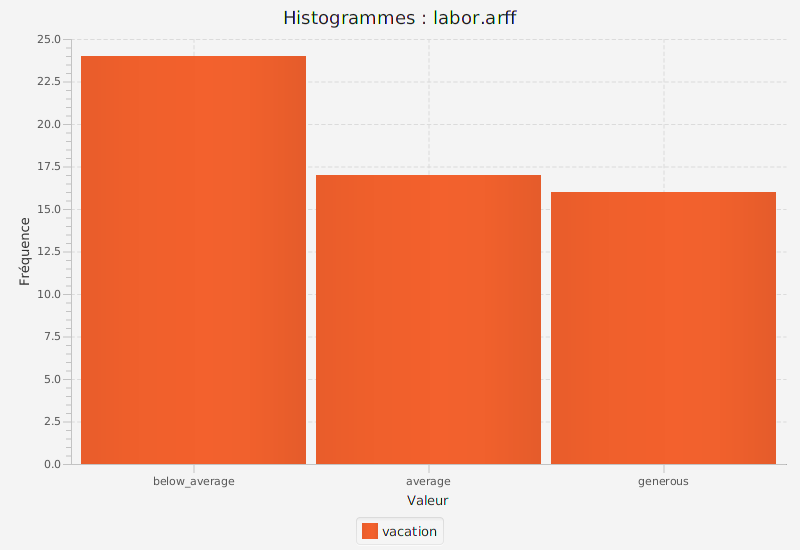
\includegraphics[width=0.8\textwidth]{screens/barchart/vacation-barchart.png}%
		\captionof{figure}{Histogramme de vacation du Data Set [labor.arff] .}\label{labelname}%
	\end{center}
	
	\subsubsection{discussion}
	$\bullet$ L'attribut vacation a trois valeurs possible \textbf{{below-average,average,generous}} , la distribution est assez uniforme  tel que  \textbf{below average} est la plus dominante avec  42\% du tout le data set labor , suivie de prés de \textbf{average} avec 30\% et \textbf{below-average} avec 28\% .\\
	\textbf{ }\\
	$\bullet$ Vacation reste quand même un attribut uni-modal avec la valeur ("below average ") comme plus fréquente.
	
	\newpage
	
	\subsection{Attribut 13 : longterm-disability-assistance }
	\subsubsection{Caractéristiques}
	Nous résumons les caractéristiques de cet attribut : "employer's help during employee longterm disability " dans le tableau ci-dessous:
	\begin{center}
		
\includegraphics[width=1\textwidth]{screens/att.png}\\ \includegraphics[width=1\textwidth]{screens/att-14.png}%
		\captionof{figure}{Attribut 13 : longterm-disability-assistance du Data Set [labor.arff] .}\label{labelname}%
	\end{center}
	La comparaison les valeurs de \textit{[Mode , Médiane , Moyenne]}, n'est pas possible vu qu'il s'agit d'un attribut nominal.
	
	\subsubsection{BarChart}
	
	\begin{center}
		\includegraphics[width=0.8\textwidth]{screens/barchart/longterm-disability-assistance-barchart.png}%
		\captionof{figure}{Histogramme de longterm-disability-assistance du Data Set [labor.arff] .}\label{labelname}%
	\end{center}
	
	\subsubsection{discussion}
	$\bullet $ L'on remarque que cet attribut peut prendre 2 valeurs possibles \textit{("yes" , "no")}. la répartition penche nettement vers le "yes", c'est à dire une seule valeur domine tout le data set .\\
	$\bullet $ D'ou l'on déduit que cet attribut est \textbf{Unimodale}, tel que mode = \textit{("yes")}.
	
	\newpage
	
	\subsection{Attribut 14 : contribution-to-dental-plan }
	\subsubsection{Caractéristiques}
	Nous résumons les caractéristiques de cet attribut : "Contribution au régime de soins dentaires" dans le tableau ci-dessous:
	\begin{center}
		\includegraphics[width=1\textwidth]{screens/att.png}\\ \includegraphics[width=1\textwidth]{screens/att-15.png}%
		\captionof{figure}{Attribut 14 : contribution-to-dental-plan du Data Set [labor.arff] .}\label{labelname}%
	\end{center}
	La comparaison les valeurs de \textit{[Mode , Médiane , Moyenne]}, n'est pas possible vu qu'il s'agit d'un attribut nominal.
	
	\subsubsection{BarChart}
	
	\begin{center}
		\includegraphics[width=0.8\textwidth]{screens/barchart/contribution-to-dental-plan-barchart.png}%
		\captionof{figure}{Histogramme de contribution-to-dental-plan du Data Set [labor.arff] .}\label{labelname}%
	\end{center}
	
	\subsubsection{discussion}
	$\bullet $ L'on remarque que cet attribut peut prendre 3 valeurs possibles \textit{("none" , "half" , "full")}. la répartition n'est pas uniforme, c'est à dire il y a une différence significative entre le nombre d'instances des les valeurs possibles.\\
	par exemple : la fréquence d'apparition de la valeur \textit{("none")} comparé à celle de la valeur \textit{("half")}.\\
	$\bullet $ Il est aussi à noter que cet attribut est \textbf{Unimodale}, tel que mode = \textit{("half")}.
	
	\newpage
	
	\subsection{Attribut 15 : bereavement-assistance }
	\subsubsection{Caractéristiques}
	Nous résumons les caractéristiques de cet attribut : "Contribution financière de l'employeur aux coûts du deuil" dans le tableau ci-dessous:
	\begin{center}
		\includegraphics[width=1\textwidth]{screens/att.png}\\ \includegraphics[width=1\textwidth]{screens/att-17.png}%
		\captionof{figure}{Attribut 15 : bereavement-assistance du Data Set [labor.arff] .}\label{labelname}%
	\end{center}
	
	La comparaison les valeurs de \textit{[Mode , Médiane , Moyenne]}, n'est pas possible vu qu'il s'agit d'un attribut nominal.
	
	\subsubsection{BarChart}
	
	\begin{center}
		\includegraphics[width=0.8\textwidth]{screens/barchart/bereavement-assistance-barchart.png}%
		\captionof{figure}{Histogramme de bereavement-assistance du Data Set [labor.arff] .}\label{labelname}%
	\end{center}
	
	\subsubsection{discussion}
	$\bullet $ L'on remarque que cet attribut peut prendre 2 valeurs possibles \textit{("yes" , "no")}.  la répartition n'est pas uniforme, c'est à dire les deux valeurs possibles n'apparaissent pas équitablement, autrement dis il y a un grand écart entre la fréquence de ces deux valeurs.\\
	$\bullet $ Il est aussi à noter que cet attribut est \textbf{Unimodale}, tel que mode = \textit{("yes")}.
	
	\newpage
	
	\subsection{Attribut 16 : contribution-to-health-plan }
	\subsubsection{Caractéristiques}
	Nous résumons les caractéristiques de cet attribut : "contribution de l'employeur au régime de santé" dans le tableau ci-dessous:
	\begin{center}
		\includegraphics[width=1\textwidth]{screens/att.png}\\ \includegraphics[width=1\textwidth]{screens/att-16.png}%
		\captionof{figure}{Attribut 16 : contribution-to-health-plan du Data Set [labor.arff] .}\label{labelname}%
	\end{center}
	
	La comparaison les valeurs de \textit{[Mode , Médiane , Moyenne]}, n'est pas possible vu qu'il s'agit d'un attribut nominal.
	
	\subsubsection{BarChart}
	
	\begin{center}
		\includegraphics[width=0.8\textwidth]{screens/barchart/contribution-to-health-plan-barchart.png}%
		\captionof{figure}{Histogramme de contribution-to-health-plan du Data Set [labor.arff] .}\label{labelname}%
	\end{center}
	
	\subsubsection{discussion}
	$\bullet $ L'on remarque que cet attribut peut prendre 3 valeurs possibles \textit{("none" , "half" , "full")}. la répartition n'est pas uniforme, c'est à dire il y'a une grande différence entre le nombre d'instances des les valeurs possibles.\\
	par exemple : la fréquence d'apparition de la valeur \textit{("none")} comparé à celle de la valeur \textit{("full")}.\\
	$\bullet $ Il est aussi à noter que cet attribut est \textbf{Unimodale}, tel que mode = \textit{("full")}.
	
	\newpage
	
	\subsection{La Class }
	\subsubsection{Caractéristiques}
	Il s'agit de la classe, qui est dans la grande majorité des cas de type nominal, car très utilisé dans la classification et clusterisation.
	
	\subsubsection{BarChart}
	$\bullet $ L'on remarque que la class peut prendre 2 valeurs possibles \textit{("bad" , "good")}.  la répartition n'est pas très uniforme, c'est à dire qu'il y a plus d'instance labellisé \textit{"good"} que celles labellisé \textit{"bad"}.\\
	
	\begin{center}
		\includegraphics[width=0.8\textwidth]{screens/barchart/class-barchart.png}%
		\captionof{figure}{Histogramme de class du Data Set [labor.arff] .}\label{labelname}%
	\end{center}
	
	
	\newpage
	
	\section{Conclusion générale}
	
	Suite à l'analyse de données qu'on a pu effectuer sur le Data Set \textbf{\textit{labor.arff}}, on se rend compte de la difficulté de la première étape du Data-Mining qui est la connaissance  le pré-traitement de nos données , la connaissance de nos celles-ci a été bénéfique afin d'avoir une idée sur la distribution de ces derniers selon les attributs : par exemple on remarque que la plupart des instances pour la plupart des attributs ont des valeurs dominantes ( mode) qui dans quelque cas couvre plus de la moitié ou encore le tiers des données .
	
	Le Data Set \textbf{\textit{labor}} est assez riche concernant les types d'attributs ,on a la moitié des attributs qui sont de type nominale (vacation,education-allowance ...) et
	l'autre partie est numérique (valeurs discrètes) (working-hours,duration..).
	
	On note bien qu'il existe quatre attributs symétriques (duration,wage-increase-second-year,wage-increase-third-year,statutory-holidays) autrement dit il garde une distribution uniforme à gauche et à droite de la médiane et la moyenne , par contre trois sont  négativement symétriques ce qui veut dire que la distribution se centre à gauche de la médiane (shift-differential,standby-pay,working-hours) et le seul attribut ayant une distribution symétrique positive est le (wage-increase-first-year) .
	
	Aussi nous avons remarqué la présence des out-liers sur trois attributs (working-hours,shift-diffirentiel,wage increase) qui se traduit par des valeurs aberrantes se trouvant loin de la répartition de la distribution de nos données.
	
	
	
	\chapter*{Bibliographie}
	
	\textbf{[1]} http://weka.sourceforge.net/doc.dev/\\
	\textbf{[2]} http://www.info.univ-angers.fr/~gh/wstat/discr.php\\
=======

\setcounter{tocdepth}{2}
\tableofcontents
\newpage
\listoffigures
\newpage

\chapter{Exploration des données}
\section{La bibliothèque WEKA [1]}
Nous avons eu recours à la bibliothèque \textbf{Weka}, en incluant \textit{weka.jar} et \textit{weka-src.jar}.
Nous avons utilisé uniquement trois (3) classes qui sont :
\begin{description}
	\item[$\bullet$ Attribute:] Elle modélise un attribut qui peut être de trois types : [numérique, nominal, String],parmi les méthodes utilisées: enumerateValues(), indexOfValue(String), isNominal(), isNumeric(), numValues(), value(position).
	  
	\item[$\bullet$ Instance:] Elle modélise une instance d'un Data Set, celle-ci ayant une valeur ou un $"?"$ pour chaque attribut, citons les méthodes utilisées : attribute(position), enumerateAttributes(), isMissing(Attribute), value(Attribute), setValue(position, double).
	
	\item[$\bullet$ Instances:] Elle représente l'ensemble de toutes les instances du Data Set, l'on à utilisé les méthodes suivante : attributeStats(position), enumerateInstances(), instance(position), numInstances(). 
\end{description}

\section{Affichage d'un DataSet}
Une liste de Data Set est accessible à partir de notre application, pour cela une liste défilante nommé \textbf{"Datasets"} est disponible sur la barre des menus.\\

Une fois un Data Set sélectionne, l'on doit appuyer sur le bouton \textbf{"Afficher"} afin qu'un tableau (instance , attribut) ne s'affiche sur la gauche de notre interface, en plus de quelques informations tel que le nombre d'instance et nombre d'attributs.\\

Mais aussi dans le cas d'un Data Set sans valeurs manquantes, une description et liste de caractéristique de chaque attribut apparaitra sur la partie droite de l'interface.

\begin{center}
	\includegraphics[width=1\textwidth]{screens/avantMissing.png}%
	\captionof{figure}{Interface de l'application affichant le Data Set [labor.arff] .}\label{labelname}%
\end{center}


\section{Remplacer les valeurs manquantes}
\subsection{but}
Remplacer les valeurs manquantes a pour principale but de redonner une certaine qualité au données, et éviter de tomber dans des cas d'inconsistance et d'incohérence par la suite dans le processus d'extraction de connaissances .

\subsection{Méthode : entièrement implémenter (Orienté classe)}

\textbf{Valeurs numériques :}

Cette première méthode a pour principe de étant donnée une instance I ayant un attribut Ai manquant et appartenant à une classe C , on devra alors remplacer la valeur manquante de Ai par la Moyenne des valeurs des instances appartenant à la Classe C ayant une valeur dans l'attribut Ai (non manquante).

\textbf{Implémentation:}

Pour l'implémentation de cette méthode on a choisit de construire un dictionnaire (index) de façon à avoir: la clé c'est la Classe, les valeurs sont les instances I ayant une valeur (non manquante ) dans l'attribut Ai.

\textbf{exemple: Dictionnaire pour l'attribut DURATION (numeric)}
\begin{center}
	\includegraphics[width=1\textwidth]{screens/dic1.png}%
	\captionof{figure}{Dictionnaire par Classe regroupant les instances dont la valeur de l'attribut DURATION existe, Data Set [labor.arff] .}\label{labelname}%
\end{center}

\textbf{exemple: Dictionnaire pour l'attribut WAGE INCREASED EACH YEAR (numeric)}
\begin{center}
	\includegraphics[width=1\textwidth]{screens/dic2.png}%
	\captionof{figure}{Dictionnaire par Classe regroupant les instances dont la valeur de l'attribut WAGE INCREASED EACH YEAR existe, Data Set [labor.arff].}\label{labelname}%
\end{center}

\textbf{Valeurs nominales:}
Pour les valeurs nominal on choisit d'exploiter notre structure de dictionnaire et pour une instance I assigner pour chaque attribut manquant Ai appartenant à une classe C, le MODE de la Classe à laquelle l'instance Appartient (Classe C).\\

\textbf{exemple: Dictionnaire pour l'attribut contribution-to-dental-plan}
\begin{center}
	\includegraphics[width=1\textwidth]{screens/dicnominal1.png}%
	\captionof{figure}{Dictionnaire pour la classe bad regroupant les instances dont la valeur de l'attribut contribution-to-dental-plan existe, Data Set [labor.arff].}\label{labelname}%
\end{center}


\begin{center}
	\includegraphics[width=1\textwidth]{screens/dicnominal.png}%
	\captionof{figure}{Dictionnaire pour la classe good regroupant les instances dont la valeur de l'attribut contribution-to-dental-plan existe, Data Set [labor.arff].}\label{labelname}%
\end{center}

 
\subsection{Résultat}
Le Data Set avant de remplacer les valeurs manquantes est comme suit: 
\begin{center}
	\includegraphics[width=1\textwidth]{screens/avantMissing.png}%
	\captionof{figure}{Data Set [labor.arff] avant traitement des valeurs manquantes.}\label{labelname}%
\end{center}

L'on remarque les points d'interrogation \textit{"?"} représentant les valeurs manquantes aussi bien pour les attributs nominaux que numériques.\\

Après avoir sélectionné dans la barre des menus l'option \textbf{Data Cleaning $>$ Missing value class} l'on obtient le résultat suivant:

\begin{center}
	\includegraphics[width=1\textwidth]{screens/apresMissing.png}%
	\captionof{figure}{Data Set [labor.arff] après traitement des valeurs manquantes.}\label{labelname}%
\end{center}

\section{Discrétisation}
\subsection{But[2]}
Discrétiser un attribut numérique (à valeurs quantitatives) c'est transformer l'ensemble des valeurs réels d'un attribut en un autre ensemble réduit d'intervalles ou de classes représentatifs du premier ensemble. On dis aussi "réaliser un découpage en classes". \\
Lorsque le nombre de valeur d'un attribut est énorme, l'affichage des histogrammes pour l'étude des caractéristiques de cet attribut est illisible, ou les informations que l'on en tire ne sont pas pertinentes, c'est pour cela que l'on à recours à la discrétisation.

\subsection{Méthode}
\subsubsection{Choix du nombre d'intervalles}

Il existe quelques formules de moindre complexité pour déterminer à l'aveugle le nombre de classes à partir de:\\
\textbf{N} : le nombre total de données.\\
\textbf{Min} : le minimum des données.\\
\textbf{Max} : le maximum des données.\\
\textbf{IQR} : l'écart inter-quartiles (paramètres de la dispersion).\\

Nous avons choisi la fonction de \textbf{Freedman-Diaconis} qui est la suivante:
\begin{center}
	$NbrIntervalle = \dfrac{Max - Min}{2 * IQR * N^{-\frac{1}{3}}}$
\end{center}

 
\subsubsection{Création des intervalles/classes}

Parmi plusieurs méthodes existantes nous avons opté pour \textbf{ La méthode des amplitudes} c'est à dire à tailles (amplitudes) égales.\\
Tel que la taille de chaque intervalle est égale à:
\begin{center}
	$Amplitude = \dfrac{(Max - Min)}{NbrIntervalle} $\\
\end{center}

\textbf{ }\\
Ainsi en le $1^{er}$ intervalle =$[Min : Min+Amplitude]$,\\
 le suivant = [$Min+Amplitude : Min+2*Amplitude$], ... 


\subsubsection{Remplacement de chaque valeur par la borne supérieur de l'intervalle au quel elle appartient}

Ainsi pour chaque attribut , nous parcourons toutes les valeurs de celui-ci et pour chacune de ses valeur nous vérifions à quel intervalle $"I"$ elle appartient, puis nous remplaçons cette valeur par la borne supérieure de $I$.\\

\underline{\textbf{PS:}} 
L'attribut étant de type numérique et afin de ne pas dénaturer la dataset, nous avons retenu uniquement la borne supérieur des intervalles pour remplacer les valeurs lors de la discrétisation.

\subsection{Résultat}
Le Data Set avant discrétisation est comme suit: 
\begin{center}
	\includegraphics[width=1\textwidth]{screens/avantDiscr.png}%
	\captionof{figure}{Data Set [labor.arff] avant discrétisation.}\label{labelname}%
\end{center}

Après avoir sélectionné dans la barre des menus l'option \textbf{Data Transformation $>$ Discrétisation} l'on obtient le résultat suivant:

\begin{center}
	\includegraphics[width=1\textwidth]{screens/apresDiscr.png}%
	\captionof{figure}{Data Set [labor.arff] après discrétisation.}\label{labelname}%
\end{center}

\underline{\textbf{Remarque}}
Nous remarquons ainsi que le degré de similitude entre les instances par rapport aux attributs est plus visible, ainsi nous espérons avoir de meilleurs résultats pour les prochaines étapes.



\section{Normalisation}
\subsection{But}

Pour la visualisation des données, et surtout la comparaison des distributions et caractéristiques des différents attributs d'un Data Set, nous avons recours à la normalisation des données de ce dernier, car les attributs des Data Set proviennent avec des ordres de grandeurs différents.\\

en plus que les attributs à grande valeur numérique influeront plus les résultats lors des traitements, apprentissage, ...

\subsection{Méthode}
Cette étape est réalisable en alignant tous les attributs sur une même plage de valeur, généralement [0:1], la formule est la suivante:
\begin{center}
	$normalisee = \dfrac{originale - MIN}{MAX - MIN}$
\end{center}
\textbf{[MIN,MAX]} : intervalle d'origine.\\
\textbf{originale} : valeur dans l'intervalle d'origine.\\
\textbf{normalisee} : valeur normalisée dans l'intervalle cible [0,1].\\




\subsection{résultat}
Le Data Set avant la normalisation est comme suit: 
\begin{center}
	\includegraphics[width=1\textwidth]{screens/avantDiscr.png}%
	\captionof{figure}{Data Set [labor.arff] avant normalisation.}\label{labelname}%
\end{center}

Après avoir sélectionné dans la barre des menus l'option \textbf{Data Transformation $>$ Normalisation} l'on obtient le résultat suivant:

\begin{center}
	\includegraphics[width=1\textwidth]{screens/apresNormal.png}%
	\captionof{figure}{Data Set [labor.arff] après normalisation.}\label{labelname}%
\end{center}

\underline{\textbf{Remarque:}}
Il est claire qu'il est plus simple de comparer les attributs une fois uniformisé, comme cela apparait dans l'affichage des boites à moustaches.






\section{Description du Data Set et de ses attributs}
Le Data Set "Labor.arff" choisi pour cette analyse comporte 16 attributs ainsi que la classe.\\
Afin de mener à bien notre étude / analyse de ce Data Set nous aurons recours à deux moyen de visualisation qui sont les Histogramme (BarChart) ainsi que les Boites à moustache (BoxPlot), ce dernier est utilisé uniquement sur les attributs numériques, et donnée par les figures ci-dessous:
\begin{center}
	\includegraphics[width=1\textwidth]{screens/BoxPlot.png}%
	\captionof{figure}{Boites à moustaches du Data Set [labor.arff] brute.}\label{labelname}%
\end{center}

\begin{center}
	\includegraphics[width=1\textwidth]{screens/BoxPlotN.png}%
	\captionof{figure}{Boites à moustaches du Data Set [labor.arff] après normalisation.}\label{labelname}%
\end{center}

\underline{\textbf{Remarque}}
Ces figures seront détaillées lors de la description des attributs.

\newpage

\subsection{Attribut 1 : duration }
\subsubsection{Caractéristiques}
Nous résumons les caractéristiques de cet attribut : "durée de l'accord" dans le tableau ci-dessous:
\begin{center}
	\includegraphics[width=1\textwidth]{screens/att-1.png}%
	\captionof{figure}{Attribut 1 : duration du Data Set [labor.arff] .}\label{labelname}%
\end{center}
On se basant sur la comparaison les valeurs de \textit{[Mode , Médiane , Moyenne] = (2 , 2 , 2.1)}, nous déduisons la dispersion des données selon cet attribut, tel qu'il est \textbf{Symétrique}.

\subsubsection{BarChart}

\begin{center}
	\includegraphics[width=0.8\textwidth]{screens/barchart/duration-barchart.png}%
	\captionof{figure}{Histogramme de duration du Data Set [labor.arff] .}\label{labelname}%
\end{center}

\subsubsection{discussion}
$\bullet $ L'on remarque que cet attribut peut prendre 4 valeurs possibles \textit{[1.0 , 2.0 , 2.25 , 3.0]}. la répartition n'est pas uniforme vu la fréquence d'apparition de la valeur \textit{[2.25]} comparé à celle de la valeur \textit{[2.0]}.\\
\textbf{ }\\
$\bullet $ Il est aussi à noter que cet attribut est \textbf{Uni-modal}, tel que mode = \textit{[2.0]}.\\
\textbf{ }\\
$\bullet $ A travers sa boite à moustache de cet attribut nous constatons une répartition pas très uniforme des données, dans le sens ou il y a une concentration des données pour les valeurs supérieurs entre [2.0 , 3.0].


\newpage


\subsection{Attribut 2 : wage-increase-first-year }
\subsubsection{Caractéristiques}
Nous résumons les caractéristiques de cet attribut : "augmentation en première année de contrat" dans le tableau ci-dessous:
\begin{center}
	\includegraphics[width=1\textwidth]{screens/att.png}\\
	\includegraphics[width=1\textwidth]{screens/att-2.png}%
	\captionof{figure}{Attribut 2 : wage-increase-first-year du Data Set [labor.arff] .}\label{labelname}%
\end{center}

On se basant sur la comparaison les valeurs de \textit{[Mode , Médiane , Moyenne] = (2.0 , 4.0 , 3.81)}, nous déduisons la dispersion des données selon cet attribut, tel qu'il est \textbf{asymétrique positivement}.

\subsubsection{BarChart}

\begin{center}
	\includegraphics[width=0.8\textwidth]{screens/barchart/wage-increase-first-year-barchart.png}%
	\captionof{figure}{Histogramme de wage-increase-first-year du Data Set [labor.arff] .}\label{labelname}%
\end{center}

\subsubsection{discussion}							
$\bullet $ L'on remarque que cet attribut peut prendre 18 valeurs possibles \textit{[2.0 , 2.1 , 2.5 , 2.8 , 3.0 , 3.5 , 3.7 , 4.0 , 4.3 , 4.419 , 4.5 , 4.6 , 5.0 , 5.7 , 6.0 , 6.4 , 6.9 , 7.0]}. la répartition n'est pas uniforme vu par exemple : la fréquence d'apparition de la valeur \textit{[7.0]} comparé à celle de la valeur \textit{[2.0]} ou de la valeur \textit{[4.5]}.\\
\textbf{ }\\
$\bullet $ Il est aussi à noter que cet attribut est \textbf{Uni-modal}, tel que mode = \textit{[2.0]}.\\
\textbf{ }\\
$\bullet $ A travers sa boite à moustache de cet attribut nous constatons une répartition plus ou moins uniforme des données, mis à part une légère tendance vers les valeurs inférieur.


\newpage


\subsection{Attribut 3 : wage-increase-second-year }
\subsubsection{Caractéristiques}
Nous résumons les caractéristiques de cet attribut : "augmentation en deuxième année de contrat" dans le tableau ci-dessous:
\begin{center}
	\includegraphics[width=1\textwidth]{screens/att.png}\\ \includegraphics[width=1\textwidth]{screens/att-3.png}%
	\captionof{figure}{Attribut 3 : wage-increase-second-year du Data Set [labor.arff] .}\label{labelname}%
\end{center}

On se basant sur la comparaison les valeurs de \textit{[Mode , Médiane , Moyenne] = (4.0 , 4.0 , 3.93)}, nous déduisons la dispersion des données selon cet attribut, tel qu'il est \textbf{symétrique}.

\subsubsection{BarChart}

\begin{center}
	\includegraphics[width=0.8\textwidth]{screens/barchart/wage-increase-second-year-barchart.png}%
	\captionof{figure}{Histogramme de wage-increase-second-year du Data Set [labor.arff] .}\label{labelname}%
\end{center}	

\subsubsection{discussion}	
$\bullet $ L'on remarque que cet attribut peut prendre 16 valeurs possibles \textit{[2.0 , 2.5 , 2.967 , 3.0 , 3.5 , 4.0 , 4.4 , 4.458 , 4.6 , 4.8 , 5.0 , 5.3 , 5.8  , 6.0 , 6.4 , 7.0]}. la répartition n'est pas uniforme vu par exemple : la fréquence d'apparition de la valeur \textit{[7.0]} comparé à celle de la valeur \textit{[4.0]}.\\
\textbf{ }\\
$\bullet $ Il est aussi à noter que cet attribut est \textbf{Uni-modal}, tel que mode = \textit{[4.0]}.\\
\textbf{ }\\
$\bullet $ La boite à moustache de cet attribut nous permet de remarquer que la distribution des valeurs n'est pas tout à fait uniforme, tel que plusieurs valeur assez grandes n'apparaissent qu'une fois dans tous le Data Set, ce qui signifie qu'elles peuvent être considérées comme des valeurs aberrantes (out-liers).

\newpage


\subsection{Attribut 4 : wage-increase-third-year }
\subsubsection{Caractéristiques}
Nous résumons les caractéristiques de cet attribut : "augmentation en troisième année de contrat" dans le tableau ci-dessous:
\begin{center}
	\includegraphics[width=1\textwidth]{screens/att.png}\\ \includegraphics[width=1\textwidth]{screens/att-4.png}%
	\captionof{figure}{Attribut 4 : wage-increase-third-year du Data Set [labor.arff] .}\label{labelname}%
\end{center}

On se basant sur la comparaison les valeurs de \textit{[Mode , Médiane , Moyenne] = (4.0 , 4.0 , 3.93)}, nous déduisons la dispersion des données selon cet attribut, tel qu'il est \textbf{symétrique}.

\subsubsection{BarChart}

\begin{center}
	\includegraphics[width=0.8\textwidth]{screens/barchart/wage-increase-third-year-barchart.png}%
	\captionof{figure}{Histogramme de wage-increase-third-year du Data Set [labor.arff] .}\label{labelname}%
\end{center}

\subsubsection{discussion}
$\bullet $ L'on remarque que cet attribut peut prendre 11 valeurs possibles \textit{[2.0 , 2.1 , 2.15 , 2.3 , 2.5 , 4 , 4.5 , 4.555 , 4.6 , 5.0 , 5.1]}. la répartition n'est pas uniforme vu par exemple : la fréquence d'apparition de la valeur \textit{[5.1]} comparé à celle de la valeur \textit{[2.15]}.\\
\textbf{ }\\
$\bullet $ Il est aussi à noter que cet attribut est \textbf{Uni-modal}, tel que mode = \textit{[4.555]}.\\
\textbf{ }\\
$\bullet $ La boite à moustache de cet attribut nous permet d'apprécier la distribution uniforme de ses valeurs, ainsi aucune valeur aberrante n'y
figure.


\newpage

\subsection{Attribut 5 : cost-of-living-adjustment }
\subsubsection{Caractéristiques}
Nous résumons les caractéristiques de cet attribut dans le tableau ci-dessous:
\begin{center}
	\includegraphics[width=1\textwidth]{screens/att.png}\\ \includegraphics[width=1\textwidth]{screens/att-5.png}%
	\captionof{figure}{Attribut 5 : cost-of-living-adjustment du Data Set [labor.arff] .}\label{labelname}%
\end{center}

\subsubsection{BarChart}
\begin{center}
	\includegraphics[width=0.8\textwidth]{screens/barchart/cost-of-living-adjustment-barchart.png}%
	\captionof{figure}{Histogramme de cost-of-living-adjustment du Data Set [labor.arff] .}\label{labelname}%
\end{center}
\subsubsection{discussion}
$\bullet$ On remarque ici facilement que la valeur la plus fréquente est la \textbf{"none"} ,avec environ 70\% du tout le data set , on retrouve \textbf{"tcf","tc"} avec seulement 12\% chacun.\\
\textbf{ }\\
$\bullet$ On peut conclure que l'attribut est \textbf{Uni-modal }(NOne est le mode et il est unique), de plus la distribution n'est pas uniforme  tel que deux valeurs \textbf{(none)} prend le dessus sur plus de 70\% de tout le Data Set.


\newpage

\subsection{Attribut 6 : working-hours }
\subsubsection{Caractéristiques}
Nous résumons les caractéristiques de cet attribut : "nombre d'heure de travail" dans le tableau ci-dessous:
\begin{center}
	\includegraphics[width=1\textwidth]{screens/att.png}\\ \includegraphics[width=1\textwidth]{screens/att-6.png}%
	\captionof{figure}{Attribut 6 : working-hours du Data Set [labor.arff] .}\label{labelname}%
\end{center}
On se basant sur la comparaison les valeurs de \textit{[Mode , Médiane , Moyenne] = (40.0 , 38.0 , 38.002)}, nous déduisons la dispersion des données selon cet attribut, tel qu'il est légèrement \textbf{asymétrique négativement}.

\subsubsection{BarChart}
\begin{center}
	\includegraphics[width=0.8\textwidth]{screens/barchart/working-hours-barchart.png}%
	\captionof{figure}{Histogramme de working-hours du Data Set [labor.arff] .}\label{labelname}%
\end{center}
\subsubsection{discussion}
$\bullet $ L'on remarque que cet attribut peut prendre 10 valeurs possibles \textit{[27.0 , 33.0 , 35.0 , 36.0 , 37.0 , 37.406 , 38.0 , 39.0 , 39.105 , 40.0]}. la répartition n'est pas uniforme vu par exemple la fréquence d'apparition de la valeur \textit{[40.0]} comparé à celle de la valeur \textit{[27.0]}.\\
\textbf{ }\\
$\bullet $ Il est aussi à noter que cet attribut est \textbf{Uni-modal}, tel que l'unique mode = \textit{[40.0]}.\\
\textbf{ }\\
$\bullet $ Aussi à partir de la boite à moustache de cet attribut, nous observons que l'ensemble des données (instances) est concentré entre [37.0 , 40.0] hors que le min est de 27h qui n'apparait qu'une seule fois, d'ailleurs se détail est bien représenté dans la boite à moustache par une flèche orange vers le bas, cela signifie la présence de valeur aberrante (out-lier). 

\newpage


\subsection{Attribut 7 : pension }
\subsubsection{Caractéristiques}
Nous résumons les caractéristiques de cet attribut : "contribution des employées à la pension" dans le tableau ci-dessous:
\begin{center}
	\includegraphics[width=1\textwidth]{screens/att.png}\\ \includegraphics[width=1\textwidth]{screens/att-7.png}%
	\captionof{figure}{Attribut 7 : pension du Data Set [labor.arff] .}\label{labelname}%
\end{center}

\subsubsection{BarChart}
\begin{center}
	\includegraphics[width=0.8\textwidth]{screens/barchart/pension-barchart.png}%
	\captionof{figure}{Histogramme de pension du Data Set [labor.arff] .}\label{labelname}%
\end{center}
\subsubsection{discussion}
$\bullet$ Comme vu plus haut l'attribut pension(contribution des employées à la pension) a trois valeurs possible (none,ret\_allw(retraité),empl\_contr), \textbf{empl\_contr} étant la plus fréquente avec  75\% , suivie de \textbf{none} (aucune valeur)
à 17\% et plus rarement (ret\_allw) ayant 4\% seulement.\\
\textbf{ }\\
$\bullet$ Pension est alors uni-modal(avec empl\_contr) qui contribue le plus  au plan pension, et les retraités beaucoup moins avec seulement 4\%, ceux qui restent ne contribuent pas du tout au plan pension (none).

\newpage

\subsection{Attribut 8 : standby-pay }
\subsubsection{Caractéristiques}
Nous résumons les caractéristiques de cet attribut : "rémunération au repos" dans le tableau ci-dessous:
\begin{center}
	\includegraphics[width=1\textwidth]{screens/att.png}\\ \includegraphics[width=1\textwidth]{screens/att-8.png}%
	\captionof{figure}{Attribut 8 : standby-pay du Data Set [labor.arff] .}\label{labelname}%
\end{center}


\subsubsection{BarChart}
\begin{center}
	\includegraphics[width=0.8\textwidth]{screens/barchart/standby-pay-barchart.png}%
	\captionof{figure}{Histogramme de standby-pay du Data Set [labor.arff] .}\label{labelname}%
\end{center}

\subsubsection{discussion}
$\bullet$ L'attribut standby-pay est numérique ,d'aprés l'histogramme de distribution des valeurs on remarque qu'il est uni-modal et la valeur la plus fréquente est de 11.4 suivie de 2.5, à noter que c'est les valeurs calculées auparavant lors des bourrages des valeurs manquantes , on peut déduire alors que avant nettoyage de données l'attribut avait pour mode 2.0 .\\
\textbf{ }\\
$\bullet$ Les valeurs de l'attribut varie entre min 2.0 jusqu'à max 14 ,en observant la boite à moustache on peut voir que la distribution des données est du coté gauche de la médiane ce qui se confirme avec moyenne < à la médiane == mode , le max 14 est ici considéré comme out-lier .
ceci nous permet de conclure que Standby-pay est un attribut positivement symétrique .

\newpage


\subsection{Attribut 9 : shift-differential }
\subsubsection{Caractéristiques}
Nous résumons les caractéristiques de cet attribut : "supplément pour travail sur les équipes II et III" dans le tableau ci-dessous:
\begin{center}
	\includegraphics[width=1\textwidth]{screens/att.png}\\ \includegraphics[width=1\textwidth]{screens/att-10.png}%
	\captionof{figure}{Attribut 9 : shift-differential du Data Set [labor.arff] .}\label{labelname}%
\end{center}

\subsubsection{BarChart}
\begin{center}
	\includegraphics[width=0.8\textwidth]{screens/barchart/shift-differential-barchart.png}%
	\captionof{figure}{Histogramme de shift-differential du Data Set [labor.arff] .}\label{labelname}%
\end{center}

\subsubsection{discussion}
$\bullet$ L'attribut shift-differential (supplément de travail sur poste 1 , 2 (travail pendant les vacances)...) est numérique ,d'après l'histogramme de distribution des valeurs on remarque facilement qu'il est uni-modal , avec 3 comme unique mode avant nettoyage des données puis 5.8 après bourrages des valeurs manquantes, par contre d'âpres la boite à moustache on observe que la distribution des données (instances) est plutôt loin des min et max qui sont de 0 et 25 respectivement. \\

25  peut être considéré comme valeur aberrante(out-lier) il n'apparaît qu'une seule fois (une seule instance) et il est très loin de la moyenne et la médiane ainsi que du mode (5.8).\\
\textbf{ }\\
$\bullet$ la médiane étant inférieur à la moyenne et la moyenne au mode  donc l'attribut a une distribution qui  est légèrement symétrique négativement tel que la plus part des données se concentre après la médiane coté gauche.


\newpage


\subsection{Attribut 10 : education-allowance}
\subsubsection{Caractéristiques}
Nous résumons les caractéristiques de cet attribut : "allocation d'éducation" dans le tableau ci-dessous:
\begin{center}
	\includegraphics[width=1\textwidth]{screens/att.png}\\ \includegraphics[width=1\textwidth]{screens/att-9.png}%
	\captionof{figure}{Attribut 10 : education-allowance du Data Set [labor.arff] .}\label{labelname}%
\end{center}

\subsubsection{BarChart}
\begin{center}
	\includegraphics[width=0.8\textwidth]{screens/barchart/education-allowance-barchart.png}%
	\captionof{figure}{Histogramme de education-allowance du Data Set [labor.arff] .}\label{labelname}%
\end{center}

 \subsubsection{discussion}
$\bullet$ L'attribut education-allowance est binaire soit oui, ou non (bourses données par l'employeur à l'employé) .On remarque que dans 84\%  des on ne donne pas d'education-allowance  par contre  seulement \%16  ont droit à une education-allowance.\\
\textbf{ }\\
$\bullet$ On conclue que "education-allowance" est uni-modal avec la valeur "NO" la plus fréquente.
 
 
\newpage

\subsection{Attribut 11 : statutory-holidays}
\subsubsection{Caractéristiques}
Nous résumons les caractéristiques de cet attribut : "nombre de jours fériés" dans le tableau ci-dessous:
\begin{center}
	\includegraphics[width=1\textwidth]{screens/att.png}\\ \includegraphics[width=1\textwidth]{screens/att-11.png}%
	\captionof{figure}{Attribut 11 : statutory-holidays du Data Set [labor.arff] .}\label{labelname}%
\end{center}

\subsubsection{BarChart}
\begin{center}
	\includegraphics[width=0.8\textwidth]{screens/barchart/statutory-holidays-barchart.png}%
	\captionof{figure}{Histogramme de statutory-holidays du Data Set [labor.arff] .}\label{labelname}%
\end{center}

\subsubsection*{discussion}


$\bullet$ L'attribut statutory holidays est representatif des nombres en jours de vacances permises, on remarque que il varie entre min=10 et max=15 , d'après la répartition des données sur l'histogramme on peut interpréter l'existence d'un seul mode qui est : 11 ce qui implique attribut $\Rightarrow$ (uni-modal) ainsi que 10 et 11 ,13 couvre plus de la moitié (prés de 77\%) de toutes la distribution des données.\\
\textbf{ }\\
$\bullet$ Maintenant à partir de la boite à moustache on peut facilement noter que la médiane et la moyenne sont égales , leur valeur étant 11 qui est aussi la valeur du mode cella nous permet de conclure que la distribution des données selon l'attribut "statutory holidays " est symétrique . (uniforme) 

\newpage

\subsection{Attribut 12 : vacation}
\subsubsection{Caractéristiques}
Nous résumons les caractéristiques de cet attribut : "nombre de jours de congés payés" dans le tableau ci-dessous:
\begin{center}
	\includegraphics[width=1\textwidth]{screens/att.png}\\ \includegraphics[width=1\textwidth]{screens/att-13.png}%
	\captionof{figure}{Attribut 12 : vacation du Data Set [labor.arff] .}\label{labelname}%
\end{center}

\subsubsection{BarChart}
\begin{center}
	\includegraphics[width=0.8\textwidth]{screens/barchart/vacation-barchart.png}%
	\captionof{figure}{Histogramme de vacation du Data Set [labor.arff] .}\label{labelname}%
\end{center}

\subsubsection{discussion}
$\bullet$ L'attribut vacation a trois valeurs possible \textbf{{below-average,average,generous}} , la distribution est assez uniforme  tel que  \textbf{below average} est la plus dominante avec  42\% du tout le data set labor , suivie de prés de \textbf{average} avec 30\% et \textbf{below-average} avec 28\% .\\
\textbf{ }\\
$\bullet$ Vacation reste quand même un attribut uni-modal avec la valeur ("below average ") comme plus fréquente.
  
  \newpage

\subsection{Attribut 13 : longterm-disability-assistance }
\subsubsection{Caractéristiques}
Nous résumons les caractéristiques de cet attribut : "employer's help during employee longterm disability " dans le tableau ci-dessous:
\begin{center}
	\includegraphics[width=1\textwidth]{screens/att.png}\\ \includegraphics[width=1\textwidth]{screens/att-14.png}%
	\captionof{figure}{Attribut 13 : longterm-disability-assistance du Data Set [labor.arff] .}\label{labelname}%
\end{center}
La comparaison les valeurs de \textit{[Mode , Médiane , Moyenne]}, n'est pas possible vu qu'il s'agit d'un attribut nominal.

\subsubsection{BarChart}

\begin{center}
	\includegraphics[width=0.8\textwidth]{screens/barchart/longterm-disability-assistance-barchart.png}%
	\captionof{figure}{Histogramme de longterm-disability-assistance du Data Set [labor.arff] .}\label{labelname}%
\end{center}

\subsubsection{discussion}
$\bullet $ L'on remarque que cet attribut peut prendre 2 valeurs possibles \textit{["yes" , "no"]}. la répartition penche nettement vers le "yes", c'est à dire une seule valeur domine tout le data set .\\
$\bullet $ Il est aussi à noter que cet attribut est \textbf{Unimodale}, tel que mode = \textit{["yes"]}.

\newpage

\subsection{Attribut 14 : contribution-to-dental-plan }
\subsubsection{Caractéristiques}
Nous résumons les caractéristiques de cet attribut : "Contribution au régime de soins dentaires" dans le tableau ci-dessous:
\begin{center}
	\includegraphics[width=1\textwidth]{screens/att.png}\\ \includegraphics[width=1\textwidth]{screens/att-15.png}%
	\captionof{figure}{Attribut 14 : contribution-to-dental-plan du Data Set [labor.arff] .}\label{labelname}%
\end{center}
La comparaison les valeurs de \textit{[Mode , Médiane , Moyenne]}, n'est pas possible vu qu'il s'agit d'un attribut nominal.

\subsubsection{BarChart}

\begin{center}
	\includegraphics[width=0.8\textwidth]{screens/barchart/contribution-to-dental-plan-barchart.png}%
	\captionof{figure}{Histogramme de contribution-to-dental-plan du Data Set [labor.arff] .}\label{labelname}%
\end{center}

\subsubsection{discussion}
$\bullet $ L'on remarque que cet attribut peut prendre 3 valeurs possibles \textit{["none" , "half" , "full"]}. la répartition n'est pas uniforme, c'est à dire il y'a une grande différence entre le nombre d'instances des les valeurs possibles.\\
par exemple : la fréquence d'apparition de la valeur \textit{["none"]} comparé à celle de la valeur \textit{["full"]}.\\
$\bullet $ Il est aussi à noter que cet attribut est \textbf{Unimodale}, tel que mode = \textit{["full"]}.

\newpage

\subsection{Attribut 15 : bereavement-assistance }
\subsubsection{Caractéristiques}
Nous résumons les caractéristiques de cet attribut : "Contribution financière de l'employeur aux coûts du deuil" dans le tableau ci-dessous:
\begin{center}
	\includegraphics[width=1\textwidth]{screens/att.png}\\ \includegraphics[width=1\textwidth]{screens/att-17.png}%
	\captionof{figure}{Attribut 15 : bereavement-assistance du Data Set [labor.arff] .}\label{labelname}%
\end{center}

La comparaison les valeurs de \textit{[Mode , Médiane , Moyenne]}, n'est pas possible vu qu'il s'agit d'un attribut nominal.

\subsubsection{BarChart}

\begin{center}
	\includegraphics[width=0.8\textwidth]{screens/barchart/bereavement-assistance-barchart.png}%
	\captionof{figure}{Histogramme de bereavement-assistance du Data Set [labor.arff] .}\label{labelname}%
\end{center}

\subsubsection{discussion}
$\bullet $ L'on remarque que cet attribut peut prendre 2 valeurs possibles \textit{["yes" , "no"]}.  la répartition est uniforme, c'est à dire les deux valeurs possibles sont toutes les deux de approximativement de même fréquence.\\
$\bullet $ Il est aussi à noter que cet attribut est \textbf{Unimodale}, tel que mode = \textit{["no"]}.

\newpage

\subsection{Attribut 16 : contribution-to-health-plan }
\subsubsection{Caractéristiques}
Nous résumons les caractéristiques de cet attribut : "contribution de l'employeur au régime de santé" dans le tableau ci-dessous:
\begin{center}
	\includegraphics[width=1\textwidth]{screens/att.png}\\ \includegraphics[width=1\textwidth]{screens/att-16.png}%
	\captionof{figure}{Attribut 16 : contribution-to-health-plan du Data Set [labor.arff] .}\label{labelname}%
\end{center}

La comparaison les valeurs de \textit{[Mode , Médiane , Moyenne]}, n'est pas possible vu qu'il s'agit d'un attribut nominal.

\subsubsection{BarChart}

\begin{center}
	\includegraphics[width=0.8\textwidth]{screens/barchart/contribution-to-health-plan-barchart.png}%
	\captionof{figure}{Histogramme de contribution-to-health-plan du Data Set [labor.arff] .}\label{labelname}%
\end{center}

\subsubsection{discussion}
$\bullet $ L'on remarque que cet attribut peut prendre 3 valeurs possibles \textit{["none" , "half" , "full"]}. la répartition n'est pas uniforme, c'est à dire il y'a une grande différence entre le nombre d'instances des les valeurs possibles.\\
par exemple : la fréquence d'apparition de la valeur \textit{["none"]} comparé à celle de la valeur \textit{["full"]}.\\
$\bullet $ Il est aussi à noter que cet attribut est \textbf{Unimodale}, tel que mode = \textit{["full"]}.

\newpage

\subsection{La Class }
\subsubsection{Caractéristiques}
Il s'agit de la classe, qui est dans la grande majorité des cas de type nominal, car très utilisé dans la classification et clusterisation.

\subsubsection{BarChart}
$\bullet $ L'on remarque que la class peut prendre 2 valeurs possibles \textit{["bad" , "good"]}.  la répartition n'est pas très uniforme, c'est à dire qu'il y a plus d'instance labellisé \textit{"good"} que celles labellisé \textit{"bad"}.\\

\begin{center}
	\includegraphics[width=0.8\textwidth]{screens/barchart/class-barchart.png}%
	\captionof{figure}{Histogramme de class du Data Set [labor.arff] .}\label{labelname}%
\end{center}


\newpage

\section{Conclusion générale}

Suite à l'analyse de données qu'on a pu effectuer sur le Data Set \textbf{\textit{labor.arff}}, on se rend compte de la difficulté de la première étape du Data-Mining qui est la connaissance  le pré-traitement de nos données , la connaissance de nos celles-ci a été bénéfique afin d'avoir une idée sur la distribution de ces derniers selon les attributs : par exemple on remarque que la plupart des instances pour la plupart des attributs ont des valeurs dominantes ( mode) qui dans quelque cas couvre plus de la moitié ou encore le tiers des données .

Le Data Set \textbf{\textit{labor}} est assez riche concernant les types d'attributs ,on a la moitié des attributs qui sont de type nominale (vacation,education-allowance ...) et
l'autre partie est numérique (valeurs discrètes) (working-hours,duration..).

On note bien qu'il existe quatre attributs symétriques (duration,wage-increase-second-year,wage-increase-third-year,statutory-holidays) autrement dit il garde une distribution uniforme à gauche et à droite de la médiane et la moyenne , par contre trois sont  négativement symétriques ce qui veut dire que la distribution se centre à gauche de la médiane (shift-differential,standby-pay,working-hours) et le seul attribut ayant une distribution symétrique positive est le (wage-increase-first-year) .

Aussi nous avons remarqué la présence des out-liers sur trois attributs (working-hours,shift-diffirentiel,wage increase) qui se traduit par des valeurs aberrantes se trouvant loin de la répartition de la distribution de nos données.



\chapter*{Bibliographie}

\textbf{[1]} http://weka.sourceforge.net/doc.dev/\\
\textbf{[2]} http://www.info.univ-angers.fr/~gh/wstat/discr.php\\
>>>>>>> 695a66c7bcabf4766b0b915ea99130588e0f2fad
\end{document}